\documentclass[12pt]{article}

\usepackage{tikz}
\usepackage{eso-pic}
\usepackage{graphicx}
\usepackage{titlesec}
\usepackage{fancyhdr}
\usepackage{float}
\usepackage{pdfpages}
\usepackage[sorting=none]{biblatex}
\usepackage{listings}
\usepackage[hidelinks]{hyperref}
\usepackage{subcaption}
\usepackage{shapepar}
\usepackage{amsmath,amssymb}
\usepackage{circuitikz}
\usepackage{pgfplots}
\pgfplotsset{compat=1.18}
\usepackage{xcolor}
\usepackage{caption}
\usepackage{setspace}
\usepackage[margin=2.5cm]{geometry}

\hypersetup{
	colorlinks=true,
	linkcolor=teal,
	filecolor=magenta,
	urlcolor=teal,
	citecolor=teal
}

\captionsetup{
	font=small,
	labelfont=bf,
	skip=6pt
}

\definecolor{codegreen}{rgb}{0,0.6,0}
\definecolor{codegray}{rgb}{0.5,0.5,0.5}
\definecolor{codepurple}{rgb}{0.58,0,0.82}
\definecolor{backcolour}{rgb}{0.96,0.96,0.94}
\definecolor{codeblue}{rgb}{0.13,0.29,0.53}
\lstdefinestyle{mystyle}{
	backgroundcolor=\color{backcolour},
	commentstyle=\color{codegreen}\itshape,
	keywordstyle=\color{codeblue}\bfseries,
	numberstyle=\tiny\color{codegray},
	stringstyle=\color{codepurple},
	basicstyle=\ttfamily\footnotesize,
	breakatwhitespace=false,
	breaklines=true,
	captionpos=b,
	keepspaces=true,
	numbers=left,
	numbersep=8pt,
	showspaces=false,
	showstringspaces=false,
	showtabs=false,
	tabsize=2,
	frame=single,
	rulecolor=\color{codegray},
	xleftmargin=12pt,
	framexleftmargin=12pt
}
\lstset{style=mystyle}

\usepackage{xepersian}
\SepMark{-} 
\setlength\headheight{34pt}
\settextfont[
Path={./font/},
Extension=.ttf,
BoldFont={irlotusbold},
Scale=1.2
]{IRLotus}
\setlatintextfont[Scale=1.1]{Times New Roman}
\setdigitfont[
Path={./font/},
Extension=.ttf,
BoldFont={Yas Bd},
ItalicFont={Yas It},
BoldItalicFont={Yas BdIt},
Scale=1
]{Yas}
\onehalfspacing

\pagestyle{fancy}
\fancyhf{}
\fancyhead[R]{میدان و امواج\quad
\includegraphics[width=1cm]{img/Logo.png}}
\fancyhead[L]{\thepage}
\renewcommand{\headrulewidth}{1pt}
\renewcommand{\footrulewidth}{0pt}

\AtBeginDocument{
	\def\chapterautorefname{فصل}
	\def\sectionautorefname{بخش}
	\def\subsectionautorefname{زیربخش}
	\def\subsubsectionautorefname{بخش}
	\def\equationautorefname{رابطهٔ}
	\def\lstlistingautorefname{برنامۀ}
	\renewcommand{\lstlistingname}{برنامه}
}

\begin{document}
	\sloppy 
	
	\defpersianfont\nast[Path={./font/}, Extension=.ttf, Scale=1.8]{IranNastaliq}

\begin{titlepage}
	\thispagestyle{empty} 
	
	\AddToShipoutPictureBG*{
		\begin{tikzpicture}[remember picture, overlay]
			\draw[line width=2pt, color=codeblue]
			([shift={(1cm,-1cm)}]current page.north west)
			rectangle
			([shift={(-1cm,1cm)}]current page.south east);
		\end{tikzpicture}
	}
	
	\begin{center}
		\vspace*{1cm}
		
\includegraphics[width=4.5cm]{img/Logo.png}
		\vspace{0.5cm}
		
		{\textcolor{codeblue}{\nast دانشگاه صنعتی خواجه نصیرالدین طوسی}}\\[0.4cm]
		{\Large\textbf{دانشکده مهندسی برق}}
		
		\vfill
		
		{\Huge\textbf{گزارش پروژه امتیازی نرم‌افزار \lr{ADS}}}\\[0.8cm]
		{\huge\textbf{درس میدان‌ها و امواج}}
		
		\vfill
		
		{\large
			\textbf{استاد درس:}\\[0.2cm]
			ـــــ
		}
		
		\vspace{1cm}
		
		{\Large
			\renewcommand{\arraystretch}{1.5}
			\begin{tabular}{|c|c|}
				\hline
				\textbf{نام و نام خانوادگی} & \textbf{شماره دانشجویی} \\
				\hline
				----- & ------ \\
				\hline

			\end{tabular}
		}
		
		\vfill
		
		{\large\textbf{تابستان ۱۴۰۵}}
	\end{center}
\end{titlepage}
	
	\newpage
	\tableofcontents
	\newpage
	
	\section{از مدار کلاسیک به دنیای موج: نقطه شروع ماجرا}
	اولین چیزی که توی درس مدار یاد می‌گیریم این است که ولتاژ روی یک سیم، در هر لحظه، همه‌جا یکسان است. این فرض تا وقتی طول موج سیگنال خیلی بزرگ‌تر از ابعاد مدار باشد کاملاً درست کار می‌کند و اصلاً هم نیازی نیست نگرانش باشیم. اما به محض این‌که پا به باند مایکروویو می‌گذاریم، قضیه عوض می‌شود: طول موج با اندازه قطعات قابل مقایسه می‌شود و همان سیم ساده، به یک خط انتقال با ولتاژ و جریانی تبدیل می‌شود که به مکان هم وابسته‌اند. در این گزارش قرار است دو موضوع را دنبال کنیم که در نگاه اول شاید بی‌ربط به نظر برسند، ولی در واقع یک داستان مشترک دارند: \textbf{خطوط انتقال مایکرواستریپ}، که پاسخ می‌دهد چطور می‌شود یک «سیم» ساخت که در فرکانس‌های گیگاهرتزی درست رفتار کند، و \textbf{پارامترهای پراکندگی}، که پاسخ می‌دهد چطور می‌شود یک نظریه مدار ساخت که در همان فرکانس‌ها هم معتبر بماند. هر دو حول یک ایده مشترک می‌چرخند: همین‌که طول موج \lr{$\lambda$} به اندازه کافی کوچک شود، دیگر نمی‌شود انتشار موج را نادیده گرفت.
	

	\section{مایکرواستریپ؛ وقتی یک نوار مسی ساده اینقدر پیچیده می‌شود}

	
	\subsection{هندسه ساده، میدان‌های شلوغ}
	
	از نظر ساخت، مایکرواستریپ یکی از ساده‌ترین خطوط انتقالی است که می‌شود تصور کرد: یک نوار رسانا به عرض \lr{$W$} و ضخامت \lr{$t$} روی یک بستر دی‌الکتریک به ضخامت \lr{$d$} و ضریب \lr{$\varepsilon_r$}، با یک صفحه زمین در زیرش. دقیقاً همین سادگی ساخت (سازگاری با فوتولیتوگرافی مدارهای چاپی و \lr{MMIC}، قابلیت پروب زدن و لحیم‌کاری، و ارزان‌تر بودن نسبت به موج‌بر ماشین‌کاری‌شده) دلیل محبوبیت زیادش شده. اما همین سادگی هندسی، سرمنشأ یک دردسر تحلیلی است: میدان الکتریکی زیر نوار مستقیم به سمت زمین می‌رود، ولی در لبه‌ها خم می‌شود و در هوا خاتمه می‌یابد  پدیده‌ای که به آن \textbf{میدان حاشیه‌ای} می‌گویند و سهم قابل توجهی از انرژی را در خودش جا می‌دهد. میدان مغناطیسی برعکس، بیشتر داخل دی‌الکتریک باقی می‌ماند.
	
	نتیجه فیزیکی مهمی که از این‌جا می‌گیریم این است که مایکرواستریپ یک محیط \textbf{ناهمگن} است: موج هم‌زمان در هوا و در بستر منتشر می‌شود. یک مد کاملاً عرضی \lr{(TEM)} به یک سرعت فاز واحد \lr{$v_p=c/\sqrt{\varepsilon_r}$} برای کل موج نیاز دارد؛ اما وقتی هیچ ضریب دی‌الکتریک یکتایی محیط را توصیف نمی‌کند، شرایط مرزی ماکسول روی مرز هوا-دی‌الکتریک فقط با ظاهر شدن مؤلفه‌های طولی کوچک \lr{$E_z, H_z$} برآورده می‌شود. پس مد واقعی مایکرواستریپ در واقع \textbf{هیبرید} است (ترکیبی از \lr{TE} و \lr{TM})، نه یک \lr{TEM} خالص.
	
	\subsection{یک ترفند نجات‌بخش: تقریب شبه‌TEM}
	
	خب حالا اگر بخواهیم دقیقاً همین مد هیبریدی را حل کنیم، کار خیلی سخت می‌شود. خوشبختانه در فرکانس‌های پایین تا متوسط، طول موج آن‌قدر بزرگ‌تر از \lr{$W$} و \lr{$d$} است که می‌شود از \lr{$E_z, H_z$} چشم‌پوشی کرد؛ به این ساده‌سازی می‌گویند \textbf{تقریب شبه‌تی‌ای‌ام} و همین است که ابزارهای کلاسیک خطوط انتقال ($Z_0$, $\beta$) را برای این ساختار غیر-\lr{TEM} قابل استفاده می‌کند.
	
	سؤالی که این‌جا پیش می‌آید این است: کدام «محیط همگن معادل» می‌تواند همان ظرفیت خازنی، سرعت فاز و امپدانس را بازتولید کند؟ جواب، \textbf{ضریب دی‌الکتریک مؤثر} است:
	
	\begin{equation}
		\varepsilon_{reff} = \frac{C}{C_{air}}
	\end{equation}
	
	که در آن \lr{$C$} ظرفیت واقعی و \lr{$C_{air}$} ظرفیت همان هندسه است اگر به‌جای دی‌الکتریک، هوا می‌گذاشتیم. از آن‌جا که میدان بین دو محیط تقسیم شده، همیشه داریم:
	
	\begin{equation}
		1 < \varepsilon_{reff} < \varepsilon_r
	\end{equation}
	
	برای خطوط عریض \lr{($W/d\gg1$)}، \lr{$\varepsilon_{reff}\to\varepsilon_r$}؛ و برای خطوط باریک \lr{($W/d\ll1$)}، \lr{$\varepsilon_{reff}\to(\varepsilon_r+1)/2$}. حالا که \lr{$\varepsilon_{reff}$} را داریم:
	
	\begin{equation}
		v_p = \frac{c}{\sqrt{\varepsilon_{reff}}}, \qquad \beta = k_0\sqrt{\varepsilon_{reff}}
	\end{equation}
	
	یعنی به‌جای دست‌وپنجه نرم کردن با یک مسئله مقدار مرزی هیبریدی، یک مسئله ساده‌تر خازنی استاتیک حل می‌کنیم و نتیجه را به‌عنوان یک خط \lr{TEM} معادل تحویل می‌دهیم. تقلبی هوشمندانه است، ولی جواب می‌دهد!
	
	\subsection{از فرمول تا امپدانس: مسیر عملی محاسبه \texorpdfstring{\lr{$Z_0$}}{Z0}}
	
	حالا که مبنای نظری دستمان آمد، وقتش رسیده چند رابطه بسته ‌ عمدتاً بر پایه نگاشت همدیس ‌ را ببینیم که برای طراحی عملی پیشنهاد شده‌اند:
	
	\begin{table}[H]
		\centering
		\caption{مقایسه مدل‌های محاسبه ضریب دی‌الکتریک مؤثر و امپدانس مشخصه}
		\renewcommand{\arraystretch}{1.3}
		\begin{tabular}{|c|c|c|c|}
			\hline
			\textbf{مدل} & \textbf{سال ارائه} & \textbf{دامنه اعتبار هندسی} & \textbf{دقت تقریبی} \\
			\hline
			\lr{Wheeler} & \lr{1965 / 1977} & فرم‌های مجانبی باریک/عریض & \lr{$\sim 1$‌$2\%$} \\
			\hline
			\lr{Schneider} & \lr{1969} & تمام مقادیر \lr{$W/d$} & مناسب، با ناپیوستگی در \lr{$W/d=1$} \\
			\hline
			\lr{Hammerstad-Jensen} & \lr{1980} & تمام مقادیر \lr{$W/d$} & بهتر از \lr{$0.2\%$} \\
			\hline
		\end{tabular}
	\end{table}
	
	از بین این‌ها، معادلات \textbf{هامرشتاد-جنسن} به‌خاطر پیوستگی کامل در کل بازه \lr{$W/d$} و دقت بالایشان، به‌نوعی استاندارد صنعتی شده‌اند و در سه گام به دست می‌آیند.
	
	\textbf{گام اول امپدانس در فضای آزاد} \lr{($\varepsilon_r=1$)}:
	
	\begin{equation}
		Z_0(\text{\lr{air}}) = \frac{\eta_0}{2\pi}\ln\left[\frac{8d}{W_e} + \frac{W_e}{4d}\right], \qquad W/d \le 1
	\end{equation}
	
	\begin{equation}
		Z_0(\text{\lr{air}}) = \eta_0\left[\frac{W_e}{d} + 1.393 + 0.667\ln\left(\frac{W_e}{d}+1.444\right)\right]^{-1}, \qquad W/d \ge 1
	\end{equation}
	
	که در آن \lr{$\eta_0\approx377\,\Omega$} و \lr{$W_e$} همان عرض مؤثر است (برای این‌که ضخامت واقعی نوار هم لحاظ شود).
	
	\textbf{گام دوم ‌ ضریب دی‌الکتریک مؤثر:}
	
	\begin{equation}
		\varepsilon_{reff} = \frac{\varepsilon_r+1}{2} + \frac{\varepsilon_r-1}{2}\left(1+\frac{12d}{W}\right)^{-1/2}
	\end{equation}
	
	خوب دقت کنید که این رابطه خودش به‌طور خودکار همان حدود فیزیکی بخش قبل را بازتولید می‌کند: $\varepsilon_r$ برای $W/d\to\infty$ و $(\varepsilon_r+1)/2$ برای $W/d\to0$.
	
	\textbf{گام سوم ‌ ترکیب نهایی:}
	
	\begin{equation}
		Z_0 = \frac{Z_0(\text{\lr{air}})}{\sqrt{\varepsilon_{reff}}}
	\end{equation}
	
	که از نظر فیزیکی هم کاملاً منطقی است: بستری با \lr{$\varepsilon_r$} بالاتر، ظرفیت خازنی را زیاد می‌کند بدون این‌که اندوکتانس محسوسی تغییر کند، پس طبیعی است که \lr{$Z_0=\sqrt{L/C}$} کم شود.
	
	\textbf{یک نکته عملی که نباید فراموش شود: ضخامت متناهی نوار.} روابط بالا فرض می‌کنند نوار بی‌نهایت نازک است؛ اما نواری با ضخامت واقعی \lr{$t$} یک ظرفیت حاشیه‌ای اضافی در لبه‌ها دارد که رفتاری شبیه یک نوار پهن‌تر از خودش نشان می‌دهد. قاعده اصلاح عرض \lr{Wheeler}، با نگاشت \lr{$W/d$} به یک عرض مؤثر \lr{$W_e/d$}، دقیقاً همین موضوع را جبران می‌کند.
	
	\subsection{وقتی \texorpdfstring{\lr{$Z_0$}}{Z0} هم ثابت نمی‌ماند: داستان پاشندگی}
	
	تا این‌جا همه چیز \textbf{استاتیک} بود، یعنی فرکانس صفر فرض شده بود. ولی وقتی فرکانس به سمت باند موج‌میلی‌متری بالا می‌رود، مایکرواستریپ یک پاشندگی واقعی از خودش نشان می‌دهد: انرژی گرایش دارد در ناحیه‌ای با کم‌ترین سرعت فاز جمع شود، یعنی به سمت بستر با \lr{$\varepsilon_r$} بالاتر کشیده می‌شود. نتیجه این‌که \lr{$\varepsilon_{reff}(f)$} یک تابع صعودی است که از مقدار استاتیک شروع می‌شود و با \lr{$f\to\infty$} به \lr{$\varepsilon_r$} میل می‌کند (که همان حد رفتار موج‌بر دی‌الکتریک همگن است). و چون \lr{$v_p$} و \lr{$Z_0$} هر دو به \lr{$\varepsilon_{reff}$} وابسته‌اند، همین وابستگی فرکانسی است که باعث اعوجاج تأخیر گروه در سیگنال‌های پهن‌باند می‌شود.
	
	چند مدل اصلی برای بیان کمّی این موضوع وجود دارد:
	
	\begin{itemize}
		\item \textbf{گتسینگر \lr{(Getsinger)}} ‌ مدار معادل تشدید \lr{LC} موازی، بیشتر برای بستر آلومینا.
		\item \textbf{ادواردز و اونز \lr{(Edwards and Owens)}} ‌ یک برازش تجربی روی بستر یاقوت، در بازه محدود.
		\item \textbf{کیرشنینگ و یانسن \lr{(Kirschning and Jansen, 1982)}} ‌ دقیق‌ترین مدل، بر پایه تحلیل مد هیبرید در حوزه طیفی، معتبر تا \lr{100 GHz} با خطای کمتر از \lr{$0.6\%$}.
	\end{itemize}
	
	\begin{equation}
		\varepsilon_{reff}(f) = \varepsilon_r - \frac{\varepsilon_r - \varepsilon_{reff}(0)}{1 + P(f)}
	\end{equation}
	
	که \lr{$P(f)$} یک تابع برازش‌شده از فرکانس نرمالیزه، نسبت \lr{$W/d$} و \lr{$\varepsilon_r$} است. رفتار \lr{$Z_0(f)$} کمی پیچیده‌تر است: معمولاً در فرکانس‌های میانی یک افت موضعی دیده می‌شود و بعد دوباره افزایش پیدا می‌کند.
	
	\subsection{سقف فرکانسی مایکرواستریپ: تا کجا می‌شود بالا رفت؟}
	
	انتشار شبه‌تی‌ای‌ام تنها مدی است که مدار برایش طراحی شده؛ اما در فرکانس بالا، مدهای انگلی هم فعال می‌شوند و چون ساختار باز است، رفتارشان بیشتر شبیه آستانه‌های نشتی است تا یک قطع سخت و تمیز:
	
	\textbf{مدهای موج سطحی صفحه دی‌الکتریک.} بستر روی صفحه زمین، عملاً معادل یک صفحه دی‌الکتریک زمین‌شده است. پایین‌ترین مد یعنی \lr{$TM_0$}، در حالت ایده‌آل اصلاً قطع ندارد، ولی وقتی ضخامت بستر به یک‌چهارم طول موج داخل دی‌الکتریک نزدیک شود، اتصال قوی‌ای بین مد اصلی و این مد رخ می‌دهد؛ نتیجه‌اش نشت انرژی و کراس‌تاک ناخواسته است.
	
	\textbf{تشدید عرضی مایکرواستریپ.} در فرکانس بالا، مقطع عرضی نوار عملاً مثل یک حفره تشدید رفتار می‌کند و پایین‌ترین تشدید وقتی رخ می‌دهد که عرض نوار تقریباً برابر نیمی از طول موج مؤثر عرضی شود.
	
	به‌عنوان یک روال طراحی، هر دو آستانه محاسبه می‌شوند و کمینه آن‌ها با یک حاشیه ایمنی، حداکثر فرکانس کاری در نظر گرفته می‌شود. یک قاعده سرانگشتی خوب: ضخامت بستر نباید از حدود \lr{$10\%$} طول موج هدایت‌شده در بالاترین فرکانس کاری فراتر برود (مثلاً برای \lr{121 GHz} روی کوارتز، ضخامت باید حدود \lr{5 mil} باشد).
	
	\subsection{انرژی کجا گم می‌شود؟ سه مکانیزم تلفات}
	
	خطوط واقعی موج را با ثابت تضعیف \lr{$\alpha$} (بر حسب \lr{Np/m}) تضعیف می‌کنند، به‌صورت \lr{$e^{-\alpha z}$}، که خودش حاصل جمع سه مکانیزم است:
	
	\begin{equation}
		\alpha = \alpha_c + \alpha_d + \alpha_r
	\end{equation}
	
	\textbf{تلفات رسانا \lr{($\alpha_c$)}} از رسانایی متناهی نوار و صفحه زمین می‌آید؛ اثر پوستی جریان را در لایه‌ای به عمق \lr{$\delta_s=\sqrt{2/(\omega\mu\sigma)}$} محدود می‌کند. قاعده اندوکتانس افزایشی ویلر \lr{(1942)} می‌تواند این تلفات را بدون محاسبه سنگین میدانی تخمین بزند؛ زبری سطح مس هم بالاتر از \lr{1 GHz} باعث افزایش \lr{$\alpha_c$} می‌شود. در کل، \lr{$\alpha_c \propto \sqrt{f}$}.
	
	\textbf{تلفات دی‌الکتریک \lr{($\alpha_d$)}} از قطبش مولکولی با تأخیر در بستر ناشی می‌شود و با \textbf{تانژانت تلفات} \lr{$\tan\delta$} بیان می‌شود. فقط همان بخشی از انرژی که واقعاً داخل بستر محبوس شده، در معرض این تلفات قرار دارد:
	
	\begin{equation}
		\alpha_d = \frac{k_0\,\varepsilon_r(\varepsilon_{reff}-1)\tan\delta}{2\sqrt{\varepsilon_{reff}}\,(\varepsilon_r-1)}
	\end{equation}
	
	و چون \lr{$\alpha_d$} خطی با فرکانس رشد می‌کند ولی \lr{$\alpha_c$} با \lr{$\sqrt{f}$}، در مایکروویو پایین تلفات رسانا غالب است و در موج‌میلی‌متری (فراتر از \lr{20}-\lr{30 GHz}) تلفات دی‌الکتریک دست بالا را می‌گیرد.
	
	\textbf{تلفات تشعشعی \lr{($\alpha_r$)}} از باز بودن ساختار ناشی می‌شود: خود خط مستقیم تشعشع ناچیزی دارد، اما هر \textbf{ناپیوستگی} (مدار باز، خمیدگی، پله) تقارن میدان را به هم می‌زند. تحلیل کلاسیک لوین \lr{(1960)} انتهای مدار باز را معادل یک روزنه تشعشعی مدل کرده بود؛ خمیدگی‌های \lr{$90^\circ$} می‌توانند تا \lr{$11\%$} توان را تلف کنند، و راه‌حل استاندارد همان \textbf{خمیدگی پخ‌زده \lr{45}درجه} است که همه‌جا استفاده می‌شود. \lr{$\alpha_r \propto f^2$} و بدترین حالتش هم روی بسترهای ضخیم با \lr{$\varepsilon_r$} پایین اتفاق می‌افتد.
	

	\section{پارامترهای S }

	
	\subsection{چرا پارامترهای \lr{Z} و \lr{Y} در مایکروویو دیگر کار نمی‌کنند}
	
	نظریه مدار فرکانس پایین یک شبکه را با پارامترهای \lr{Z}، \lr{Y} یا \lr{h} بر حسب ولتاژ و جریان کل هر پورت توصیف می‌کند و برای این کار به اعمال \textbf{اتصال کوتاه} یا \textbf{مدار باز} ایده‌آل نیاز دارد. این چارچوب در مایکروویو به سه دلیل فیزیکی از هم می‌پاشد:
	
	\begin{enumerate}
		\item \textbf{ولتاژ و جریان دیگر یکتا نیستند:} در مدهای هیبرید یا غیر \lr{TEM}، انتگرال میدان الکتریکی روی یک مسیر به خود مسیر وابسته می‌شود؛ اصلاً مفهوم ولتاژ اسکالر روی یک گره دیگر معنا ندارد.
		\item \textbf{شرایط مرزی ایده‌آل عملاً غیرقابل‌تحقق‌اند:} یک اتصال کوتاه فیزیکی همیشه اندوکتانس غیرصفر دارد و در فرکانس بالا خودش شبیه مدار باز می‌شود؛ یک مدار باز فیزیکی هم به‌خاطر میدان حاشیه‌ای و تشعشع، مثل یک خازن یا یک آنتن ضعیف رفتار می‌کند.
		\item \textbf{قطعات فعال ناپایدار می‌شوند:} اتصال کوتاه یا مدار باز عمدی روی پورت یک قطعه فعال، تقریباً تمام انرژی را برمی‌گرداند و خطر نوسان ناخواسته حین اندازه‌گیری را با خودش می‌آورد.
	\end{enumerate}
	
	\subsection{راه‌حل: امواج توان رونده}
	
	کوروکاوا \lr{(Kurokawa, 1965)} پیشنهاد داد که شبکه‌ها را با \textbf{امواج توان رونده} توصیف کنیم. برای پورت \lr{$n$} با امپدانس مرجع \lr{$Z_0$} و ولتاژ/جریان \lr{$V_n,I_n$}:
	
	\begin{equation}
		a_n = \frac{V_n + Z_0 I_n}{2\sqrt{Z_0}}, \qquad b_n = \frac{V_n - Z_0 I_n}{2\sqrt{Z_0}}
	\end{equation}
	
	\lr{$a_n$} موجی است که به \textit{درون} پورت می‌رود و \lr{$|a_n|^2$} توان در دسترس از منبع را نشان می‌دهد؛ \lr{$b_n$} موج \textit{بیرون رونده} است و \lr{$|b_n|^2$} توان تحویلی به بار. برای یک خاتمه ایده‌آل \lr{($b_n=0$)}، فقط کافی است پورت به \lr{$Z_0$} خودش ختم شود (مثلاً یک بار \lr{$50\,\Omega$}) دیگر نیازی به اتصال کوتاه یا مدار باز نیست.
	
	\subsection{ماتریس \lr{S} برای یک شبکه \lr{N}-پورته}
	
	هر شبکه خطی \lr{$N$} پورته را می‌شود با نگاشت خطی زیر مشخص کرد:
	
	\begin{equation}
		[b] = [S][a]
	\end{equation}
	
	هر درایه هم با تحریک یک پورت و خاتمه‌دادن بقیه پورت‌ها با بار تطبیق‌یافته به دست می‌آید:
	
	\begin{equation}
		S_{ij} = \left.\frac{b_i}{a_j}\right|_{a_k=0,\ k\neq j}
	\end{equation}
	
	که دقیقاً همان روال عملی اندازه‌گیری با یک آنالایزور شبکه برداری \lr{(VNA)} است.
	
	\subsection{این پارامترها یعنی چه: معنای فیزیکی \texorpdfstring{\lr{$S_{11}, S_{21}, S_{12}, S_{22}$}}{S-Parameters}}
	
	برای یک شبکه دوپورته:
	
	\begin{equation}
		\begin{bmatrix} b_1 \\ b_2 \end{bmatrix} = \begin{bmatrix} S_{11} & S_{12} \\ S_{21} & S_{22} \end{bmatrix}\begin{bmatrix} a_1 \\ a_2 \end{bmatrix}
	\end{equation}
	
	\begin{itemize}
		\item \textbf{$S_{11}$:} ضریب بازتاب ورودی ‌ یعنی امپدانس پورت ۱ چقدر خوب تطبیق شده.
		\item \textbf{$S_{21}$:} ضریب انتقال مستقیم ‌ همان بهره تقویت‌کننده یا انتقال باند عبور فیلتر.
		\item \textbf{$S_{12}$:} ضریب انتقال معکوس ‌ نشت خروجی به ورودی؛ در تحلیل پایداری قطعات فعال خیلی مهم است.
		\item \textbf{$S_{22}$:} ضریب بازتاب خروجی ‌ کیفیت تطبیق در پورت ۲.
	\end{itemize}
	
	\subsection{یک چیز رایگان: تقابل‌پذیری و بدون‌تلفاتی}
	
	\textbf{شبکه‌های تقابل‌پذیر.} یک شبکه \lr{(reciprocal)} است اگر پاسخ انتقالی از پورت ۱ به ۲ با پاسخ معکوسش برابر باشد؛ این نتیجه‌ی مستقیم \textbf{قضیه تقابل‌پذیری لورنتس} است (برقرار وقتی محیط فاقد فریت مغناطیس‌شده یا پلاسمای بایاس‌دار باشد):
	
	\begin{equation}
		[S] = [S]^T \quad \Rightarrow \quad S_{ij} = S_{ji}
	\end{equation}
	
	تقریباً هر شبکه منفعل معمولی مایکرواستریپ (تقسیم‌کننده، فیلتر، خط ساده) تقابل‌پذیر است، و همین بعداً کارمان را در خواندن نتایج شبیه‌سازی راحت‌تر می‌کند.
	
	\subsection{از پارامترهای \lr{S} تا اعدادی که واقعاً روی گزارش می‌نویسیم}
	
	\textbf{تلفات بازگشتی \lr{(RL)}:}
	
	\begin{equation}
		RL = -20\log_{10}|S_{11}|\ \text{dB}
	\end{equation}
	
	\textbf{تلفات درج \lr{(IL)}:}
	
	\begin{equation}
		IL = -20\log_{10}|S_{21}|\ \text{dB}
	\end{equation}
	
	برای یک فیلتر ایده‌آل در باند عبور، \lr{$|S_{21}|\approx1$} و در نتیجه \lr{$IL\approx0$ dB}.
	
	\textbf{نسبت موج ایستاده ولتاژ \lr{(VSWR)}:}
	
	\begin{equation}
		VSWR = \frac{1+|S_{11}|}{1-|S_{11}|}
	\end{equation}
	
	مقدار ایده‌آل \lr{$VSWR=1$} است، یعنی بازتاب صفر  دقیقاً همان چیزی که در ادامه گزارش دنبالش هستیم.
	
	

	\section{جمع‌بندی}

	
	اگر بخواهم این دو بخش را در یک جمله کنار هم بگذارم: هر دو، یک حرکت فکری مشترک را طی کردند. نظریه مایکرواستریپ یک مسئله مقدار مرزی هیبریدی سخت را با تقریب شبه‌تی‌ای‌ام رام کرد و دقت کامل را با یک تصویر محیط همگن معادل معاوضه کرد معاوضه‌ای که پاشندگی و مدهای مرتبه بالاتر هر از گاهی حدش را به ما یادآوری می‌کنند. نظریه پارامترهای پراکندگی هم دقیقاً همین کار را کرد: واقعیت فروپاشی مفهوم ولتاژ و جریان در مایکروویو را با بازتعریف متغیرهای بنیادین حول امواج توان رونده حل کرد. خلاصه‌اش این‌که: هر وقت تصویر کلاسیک فرکانس پایین به‌خاطر انتشار موج از هم می‌پاشد، یک نظریه تازه دور خود موج ساخته می‌شود همین است معنای واقعی «عنصر توزیع‌شده» در مهندسی مایکروویو. و از این‌جا به بعد، وقتش رسیده این تئوری را واقعاً روی \lr{ADS} پیاده کنیم و ببینیم عملاً چه اتفاقی می‌افتد.
	
	\clearpage
	\section{وارد \lr{ADS} می‌شویم: اولین تست واقعیت}
	
	قبل از این‌که سراغ طراحی فیزیکی شبکه تطبیق برویم، منطقی‌تر است اول یک قدم کوچک‌تر برداریم: مطمئن شویم زیرلایه‌ای که انتخاب کرده‌ایم و ابعادی که برایش محاسبه شده‌اند، واقعاً درست کار می‌کنند. برای همین، یک خط انتقال استاندارد ۵۰ اهمی در فرکانس کاری ۹ گیگاهرتز می‌سازیم و تست می‌کنیم. این مرحله شاید در نگاه اول اضافی به نظر برسد، اما اگر همین‌جا یک خطای بازتاب کوچک در مسیرهای پایه یا پدهای اتصال باقی بماند، بعداً وقتی مدار پیچیده‌تر شود پیدا کردنش خیلی سخت‌تر خواهد بود.
	
	\subsection{اول از همه: زیرلایه رو درست تنظیم کنیم}
	برای پیاده‌سازی فیزیکی این مدار، از زیرلایه استاندارد \lr{RT5880} استفاده کردم. پارامترهای دقیق این زیرلایه را در بلوک \lr{MSUB} محیط شماتیک نرم‌افزار \lr{ADS} این‌طور تنظیم کردم تا شرایط شبیه‌سازی تا حد امکان با واقعیت یکی باشد:
	\begin{itemize}
		\item ثابت دی‌الکتریک نسبی (\lr{Er}): $2.2$
		\item ضخامت زیرلایه (\lr{H}): $20 \text{ mil}$
		\item ضخامت فلز مس (\lr{T}): $0.7 \text{ mil}$
		\item تانژانت تلفات دی‌الکتریک (\lr{TanD}): $0.0009$
		\item نفوذپذیری مغناطیسی نسبی (\lr{Mur}): $1$
		\item رسانایی هادی (\lr{Cond}): $1.0\times 10^{50}\ \text{S/m}$
		\item ارتفاع محفظه فلزی بالای مدار (\lr{Hu}): $1\times 10^{33}\ \text{mm}$
		\item زبری سطح هادی (\lr{Rough}): $0\ \text{mm}$
	\end{itemize}
	
	هر کدام از این پارامترها نقش فیزیکی مشخصی در دقت مدل‌سازی خط مایکرواستریپ دارند که ارزش دارد کمی بازشان کنم:
	
	\paragraph{نفوذپذیری مغناطیسی نسبی (\lr{Mur=1}):} این مقدار یعنی زیرلایه \lr{RT5880} یک ماده دی‌الکتریک غیرمغناطیسی است، پس هیچ تلفات یا اعوجاج فازی ناشی از پاسخ مغناطیسی ماده در مدل حساب نمی‌شود؛ این فرض برای تقریباً تمام زیرلایه‌های تجاری \lr{PTFE}/سرامیکی کاملاً معتبر است.
	
	\paragraph{رسانایی هادی (\lr{Cond=1.0E+50}):} این عدد عملاً معادل رسانایی بی‌نهایت (یعنی یک هادی ایده‌آل) است و به‌طور خاص تلفات اهمی هادی (\lr{Conductor Loss}) ناشی از رسانایی محدود مس واقعی را از مدل حذف می‌کند. نکته مهمش این است که در چنین شرایطی، \textbf{تنها منبع تلفاتی که در شبیه‌سازی دیده می‌شود، تلفات دی‌الکتریک زیرلایه (بر مبنای \lr{TanD}) است}؛ این ساده‌سازی برای مرحله اعتبارسنجی اولیه امپدانس مشخصه (تمرکز روی $S_{11}$) کاملاً قابل قبول است، اما اگر بخواهیم تلفات درج ($S_{21}$) خط را هم دقیق ببینیم، باید مقدار واقعی رسانایی مس ($\sigma_{Cu}\approx 5.8\times10^{7}\ \text{S/m}$) را جایگزین این عدد آرمانی کنیم.
	
	\paragraph{ارتفاع محفظه فلزی (\lr{Hu=1e+33 mm}):} این پارامتر ارتفاع یک صفحه فلزی فرضی (\lr{Enclosure/Cover}) بالای مدار مایکرواستریپ را تعریف می‌کند که در تحلیل‌های کاواک بسته کاربرد دارد. با گذاشتن یک عدد نجومی (عملاً بی‌نهایت) برایش، فاصله این سرپوش فرضی از سطح مدار آن‌قدر زیاد فرض می‌شود که هیچ جفت‌شدگی الکترومغناطیسی یا تشدید کاواکی بین میدان‌های اطراف نوار هادی و محفظه اتفاق نمی‌افتد؛ به بیان ساده‌تر، این تنظیم معادل یک فضای باز و نامحدود (\lr{Open/Unbounded Radiation Boundary}) بالای زیرلایه است دقیقاً همان چیزی که در یک برد مدار چاپی بدون محفظه فلزی واقعاً اتفاق می‌افتد.
	
	\subsection{\lr{LineCalc} و یک اشتباه واحدی که نزدیک بود کل کار رو خراب کند}
	با امپدانس مشخصه هدف ($Z_0 = 50 \ \Omega$) و فرکانس کاری ($f = 9 \text{ GHz}$)، از ابزار \lr{LineCalc} برای تبدیل این مشخصات الکتریکی به ابعاد فیزیکی خط مایکرواستریپ (\lr{MLIN}) استفاده کردم. خروجی ابزار، عرض خط را برابر با $W = 60.77 \text{ mil}$ محاسبه کرد و طول خط را هم برای آزمون مسیر انتقال $L = 10 \text{ mm}$ در نظر گرفتم. 
	
	راستش این‌جا یک اشتباه کوچک ولی مهم مرتکب شدم که ارزش گفتن دارد: اولین باری که این مقدار عرض را در قطعه \lr{MLIN} وارد کردم، بدون توجه واحد را روی \lr{mm} گذاشتم، در حالی‌که \lr{LineCalc} خروجی را بر حسب \lr{mil} داده بود. نتیجه‌اش این شد که عملاً یک خط با عرض چند برابر مقدار درست ساختم و طبیعتاً امپدانس مشخصه‌اش دیگر هیچ ربطی به \lr{$50\ \Omega$} نداشت. بعد از چک کردن دوباره تنظیمات \lr{MLIN} و مقایسه واحد فیلد \lr{W} با خروجی \lr{LineCalc}، مشکل مشخص شد و با تغییر واحد به \lr{mil} حل شد. این تجربه به من یاد داد که رعایت یکپارچگی واحدها در پارامترهای قطعه \lr{MLIN} چقدر حیاتی است، چون کوچک‌ترین خطای واحد می‌تواند امپدانس خط را به‌شدت تغییر بدهد و عملکرد کل شبکه را در محیط \lr{Layout} خراب کند.
	
	\subsection{بستن شماتیک: پورت‌ها، \lr{MSUB} و \lr{MLIN}}
	چیدمان مدار شامل پورت‌های ورودی و خروجی مجهز به ترمینال زمین (\lr{TermG}) با امپدانس مرجع $50\ \Omega$، بلوک زیرلایه \lr{MSUB} و قطعه خط مایکرواستریپ (\lr{MLIN}) با عرض درست‌شده، در شکل \ref{fig:schematic_validation} دیده می‌شود.
	
	\begin{figure}[H]
		\centering
		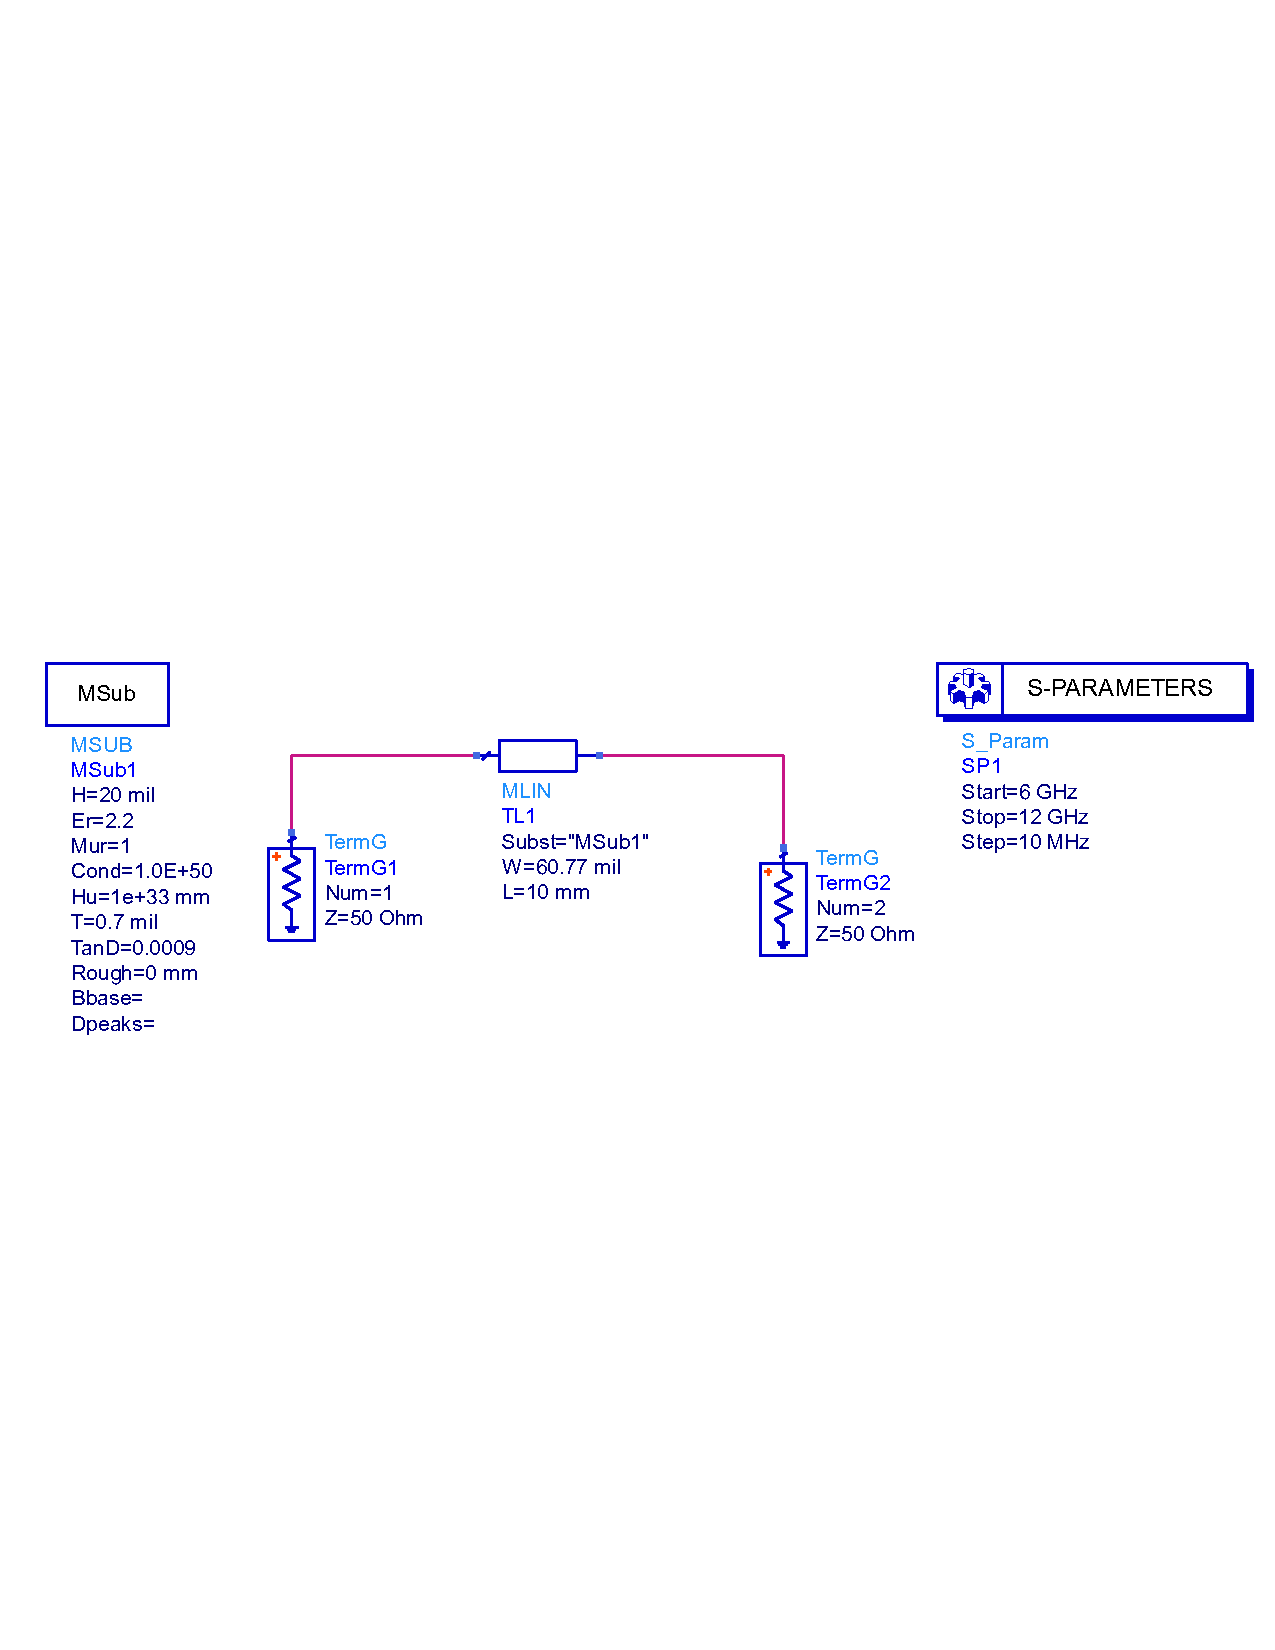
\includegraphics[trim=0 10cm 0 10cm, clip, width=0.9\textwidth]{./img/validation_shematic.pdf}
		\caption{شماتیک مدار خط انتقال ۵۰ اهم با ابعاد فیزیکی اصلاح‌شده در نرم‌افزار \lr{ADS}}
		\label{fig:schematic_validation}
	\end{figure}
	
	\subsection{اجرای اول: یک خروجی خالی و یک بلوک \lr{SP} غیرفعال}
	با شماتیک آماده، شبیه‌سازی پارامترهای \lr{S-Parameters} را در بازه فرکانسی ۶ تا ۱۲ گیگاهرتز و با گام فرکانسی $\text{Step}=10\ \text{MHz}$ (برای این‌که نقطه تشدید به‌اندازه کافی واضح دیده شود) تنظیم کردم و اجرا زدم. اولین باری که \lr{Simulate} را زدم، هیچ نموداری باز نشد و دیتاست خروجی هم عملاً خالی بود نه پیغام خطای واضحی، نه هیچ داده‌ای برای رسم. بعد از چند دقیقه گشتن، فهمیدم که در همان مرحله چیدن شماتیک، بدون توجه بلوک \lr{S\_Param} را یک بار جابه‌جا کرده بودم و ناخواسته با کلید میانبر غیرفعالش (\lr{Deactivate}) کرده بودم؛ در نتیجه شبیه‌ساز اصلاً هیچ کنترلری برای اجرای آنالیز پیدا نمی‌کرد. با فعال کردن دوباره بلوک \lr{SP1} همه چیز به حالت عادی برگشت.
	
	بعد از رفع این مشکل، نتایج نشان دادند که مقدار پارامتر $S_{11}$ در فرکانس مرکزی و هدف ۹ گیگاهرتز، دقیقاً برابر با $-73.879 \text{ dB}$ است (مطابق شکل \ref{fig:s11_validation}). این افت شدید در بازتاب سیگنال، یعنی تطبیق امپدانسی خط انتقال با پورت‌های ۵۰ اهمی فوق‌العاده خوب است. این نتیجه صحت مقادیر وارد شده برای زیرلایه و ابعاد محاسبه‌شده را کاملاً تأیید کرد و خیالم راحت شد که می‌شود وارد فاز بعدی، یعنی جایگذاری استاب‌ها و خطوط سری شبکه تطبیق، شد.
	
	\begin{figure}[H]
		\centering
		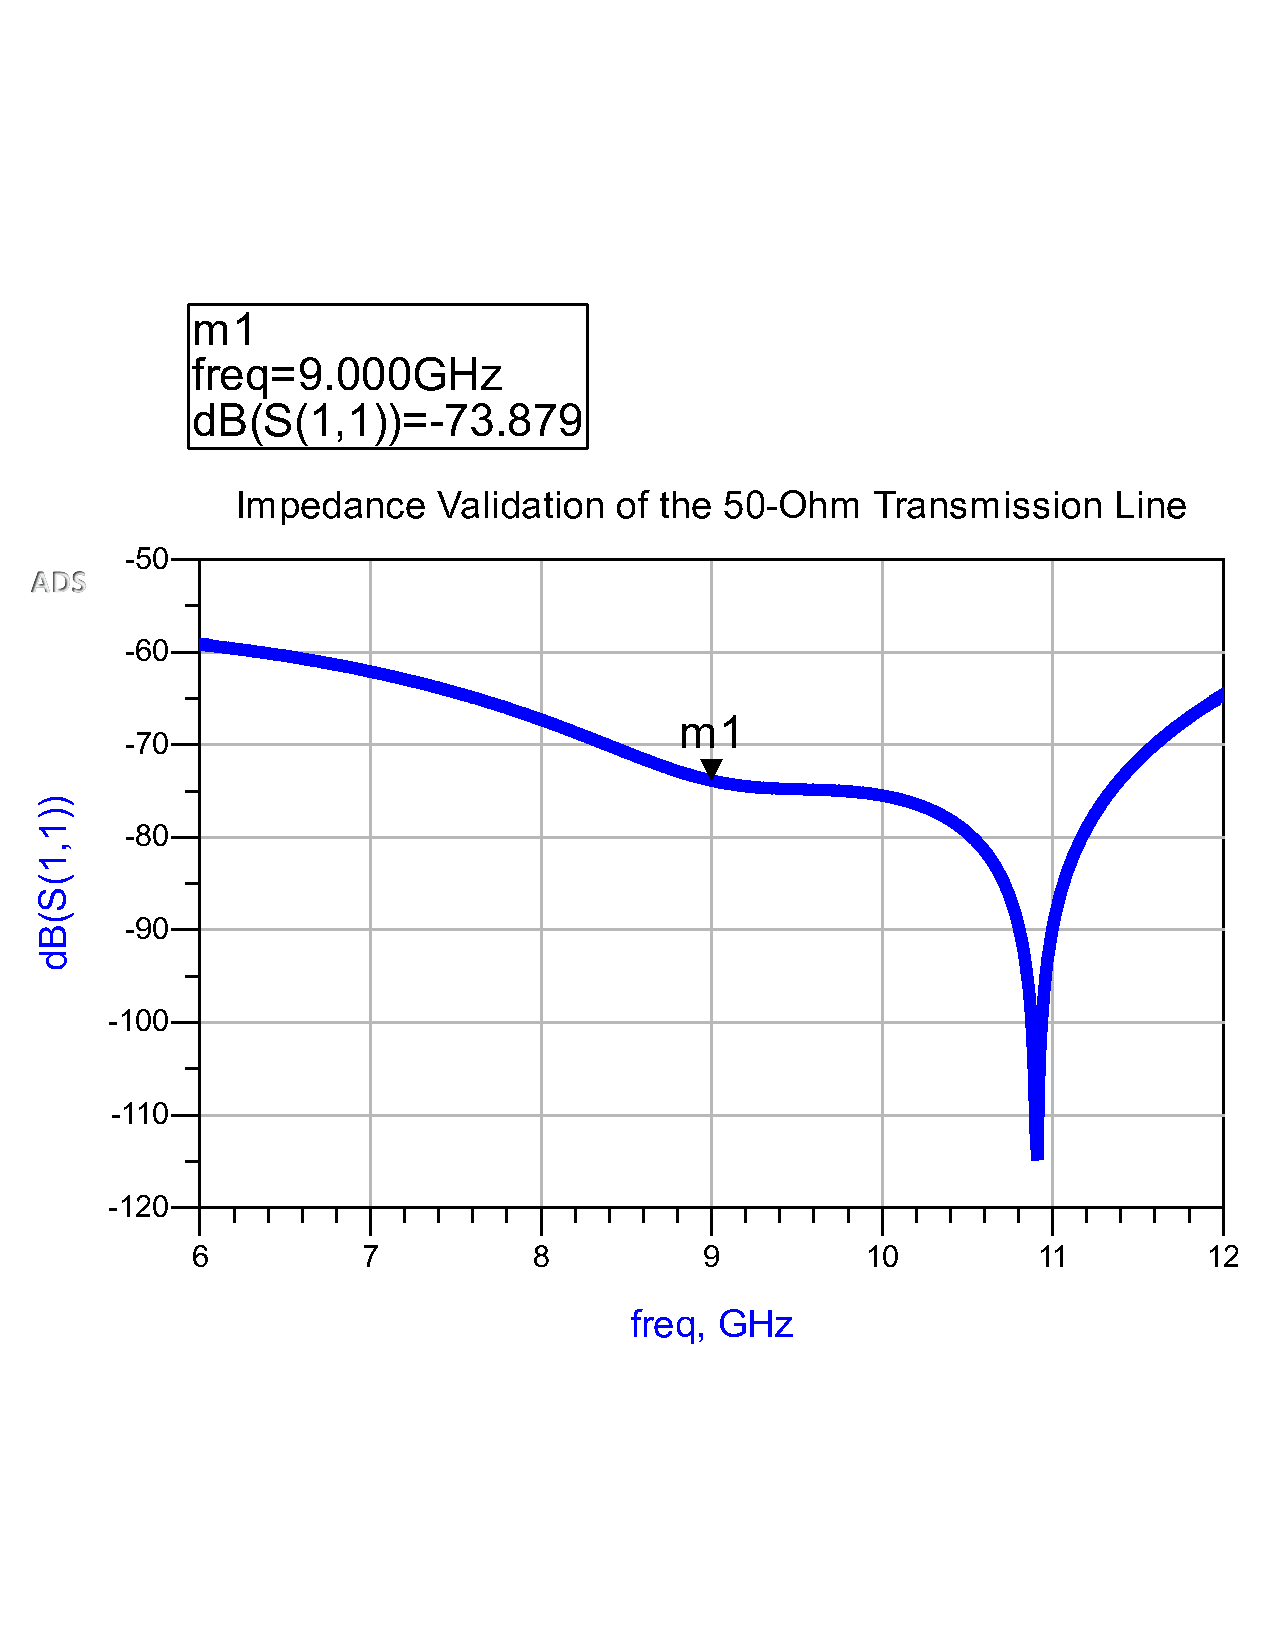
\includegraphics[trim=0 5cm 0 5cm, clip,width=0.9\textwidth]{./img/validation} 
		\caption{نمودار اندازه $S_{11}$ جهت اعتبارسنجی خط انتقال ۵۰ اهم روی زیرلایه \lr{RT5880}}
		\label{fig:s11_validation}
	\end{figure}
	
	\clearpage
	
	
	\subsection{وقت طراحی شبکه تطبیق: اسمیت چارت به کمک می‌آید}
	
	بعد از این‌که مقادیر تئوری شبکه‌های تطبیق را محاسبه کردم، برای پیاده‌سازی و اعتبارسنجی‌شان در \lr{ADS}، از ابزار داخلی نمودار اسمیت استفاده کردم. از منوی اصلی نرم‌افزار مسیر \lr{Tools > Smith Chart} را انتخاب کردم تا محیط گرافیکی و تعاملی طراحی باز شود. برای هر یک از دو شبکه (ورودی و خروجی) به‌طور جداگانه، اول فرکانس کاری را روی \lr{9 GHz} و امپدانس مرجع (\lr{Z0}) را روی 
 تنظیم کردم و بعد امپدانس‌های 
	مبدأ و مقصد هر شبکه را مطابق چیزی که در ادامه شرح می‌دهم تعریف کردم. هدف در هر دو شبکه، رسیدن به تطبیق مزدوج (\lr{Conjugate Match}) بین امپدانس مرجع$\ \Omega$	\lr{50} سیستم و امپدانس ورودی/خروجی ترانزیستور است، تا بیشینه انتقال توان در فرکانس مرکزی \lr{9 GHz} تضمین شود.
	
	با توجه به این‌که پیاده‌سازی فیزیکی استاب اتصال‌کوتاه در فناوری مایکرواستریپ عملاً امکان‌پذیر نیست، در هر دو شبکه، مسیر تطبیق را با ترکیب یک قطعه \textbf{خط انتقال سری} \lr{(Series Transmission Line)} و یک \textbf{استاب موازی مدار باز} \lr{(Open-Circuit Shunt Stub)} طراحی کردم.
	
	\subsection{شبکه ورودی: از \texorpdfstring{\lr{$Z_{in}$}}{Zin} تا مرکز نمودار}
	
	هدف شبکه تطبیق ورودی این است که امپدانس ورودی ترانزیستور را به امپدانس مرجع منبع سیگنال ($Z_0 = 50\ \Omega$) ببرد. چون امپدانس ورودی ترانزیستور برابر با
	\[
	Z_{in} = 18 - j32.1\ \Omega
	\]
	به دست آمده بود، در محیط اسمیت چارت این نقطه را به‌عنوان مبدأ حرکت پلات کردم و مقصد را هم مرکز نمودار (نقطه $50\ \Omega$) گذاشتم.
	
	راستش کار روی این ابزار اولش یک‌کم گیج‌کننده بود، چون دو تیک‌باکس \lr{Lock Source Impedance} و \lr{Lock Load Impedance} وجود دارند که خیلی واضح توضیح نمی‌دهند دقیقاً چه چیزی را قفل می‌کنند (شکل \ref{fig:smith_input}). وقتی برای شبکه ورودی این دو تیک‌باکس را نزده رها کردم در دفعه اول اشتباهیی هعی این مقادیر را روی نمودار جابجا میکردم. باید تیک رو فعال میکردم تا ثابت قفل شوند.
	
	مسیر حرکت روی نمودار اسمیت برای رسیدن از نقطه $Z_{in}$ به مرکز نمودار این‌طور طی شد: از نقطه $Z_{in}$ شروع کردم، اول یک استاب موازی مدار باز به مدار اضافه کردم تا با تغییر سوسپتانس، نقطه موردنظر روی دایره مقاومت ثابتِ گذرنده از مرکز نمودار قرار بگیرد؛ بعد با اضافه کردن یک خط انتقال سری، فاز مسیر را طوری چرخاندم که نقطه نهایی دقیقاً روی مرکز نمودار (امپدانس $50\ \Omega$) بنشیند. محیط طراحی و توپولوژی نهایی این شبکه (بلوک \lr{SmartComponent} با نام \lr{DA\_SmithChartMatch1}) در شکل \ref{fig:smith_input} نشان داده شده.
	
	\begin{figure}[H]
		\centering
		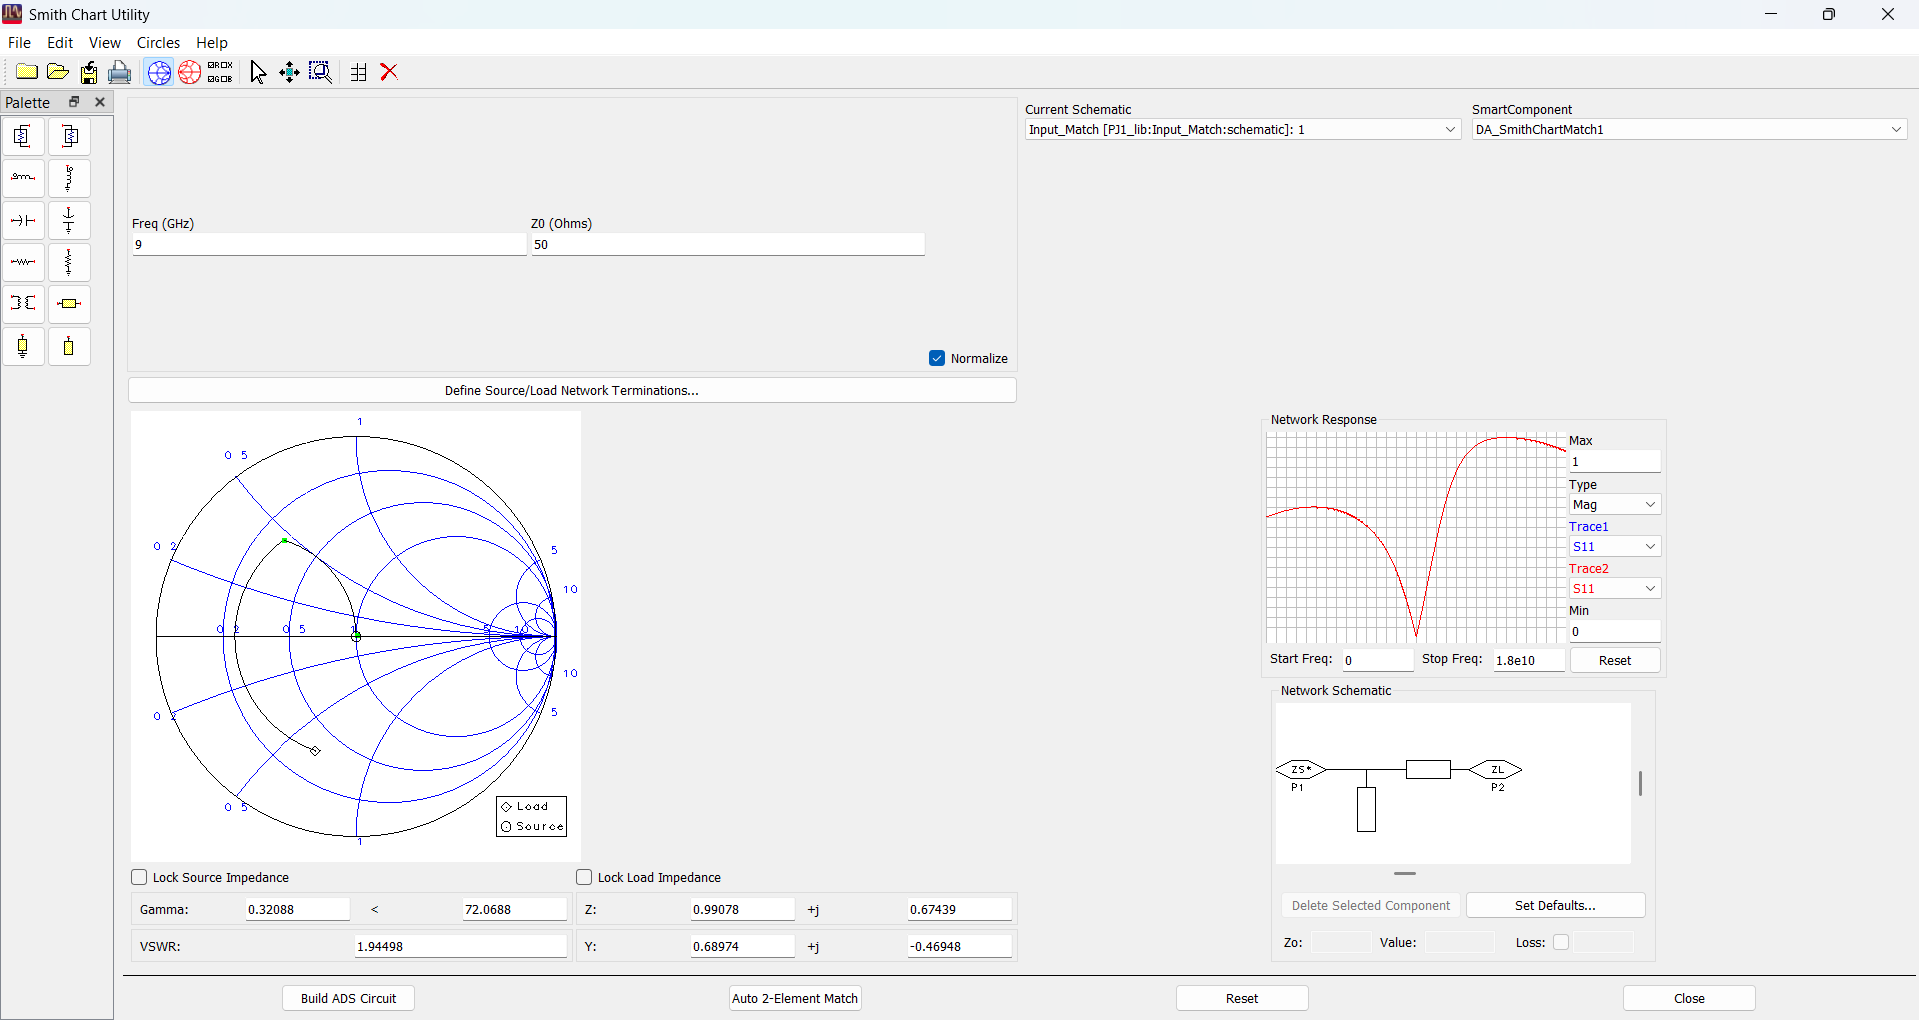
\includegraphics[width=0.8\textwidth]{./img/smith_chart_input.png}
		\caption{محیط طراحی شبکه تطبیق ورودی در ابزار \lr{Smith Chart} نرم‌افزار \lr{ADS}؛ توپولوژی شامل یک خط انتقال سری و یک استاب موازی مدار باز است}
		\label{fig:smith_input}
	\end{figure}
	
	\subsection{شبکه خروجی: دنبال مزدوج \texorpdfstring{\lr{$Z_{out}$}}{Zout}}
	
	به همین ترتیب، هدف شبکه تطبیق خروجی این است که بار $50\ \Omega$ سیستم را به امپدانس مزدوج خروجی ترانزیستور تبدیل کند. چون امپدانس خروجی ترانزیستور برابر با $Z_{out} = 49.1 - j34.3\ \Omega$ به دست آمده بود، مقدار هدف را برابر
	\[
	Z_{out}^{*} = 49.1 + j34.3\ \Omega
	\]
	گذاشتم. این‌جا برخلاف شبکه ورودی، مبدأ حرکت در نمودار اسمیت خود مرکز نمودار (نقطه $50\ \Omega$) بود و نقطه مقصد روی $Z_{out}^{*} = 49.1 + j34.3\ \Omega$ تنظیم شد. این‌بار چون هم امپدانس مبدأ و هم امپدانس مقصد از قبل مشخص و ثابت بودند، هر دو تیک‌باکس \lr{Lock Source Impedance} و \lr{Lock Load Impedance} را زدم (همان‌طور که در شکل \ref{fig:smith_output} دیده می‌شود) تا ابزار در حین اضافه کردن قطعات، این دو نقطه را جابه‌جا نکند و فقط مسیر بین‌شان را با قطعات جدید بسازد همان چیزی که برای شبکه ورودی نیازی نبود انجامش بدهم.
	
	مسیر حرکت روی نمودار اسمیت برای رسیدن به نقطه تطبیق خروجی هم شبیه شبکه ورودی طی شد: اول یک خط انتقال سری به مدار اضافه کردم تا با یک چرخش روی دایره‌ها، به دایره رسانایی ثابتِ گذرنده از نقطه هدف برسم؛ بعد در گام دوم، با اضافه کردن یک استاب موازی از نوع مدار باز، سوسپتانس را طوری تنظیم کردم که نقطه نهایی دقیقاً روی امپدانس $49.1 + j34.3\ \Omega$ بنشیند. محیط طراحی و توپولوژی نهایی این شبکه (بلوک \lr{SmartComponent} با نام \lr{DA\_SmithChartMatch2}) در شکل \ref{fig:smith_output} دیده می‌شود.
	
	\begin{figure}[H]
		\centering
		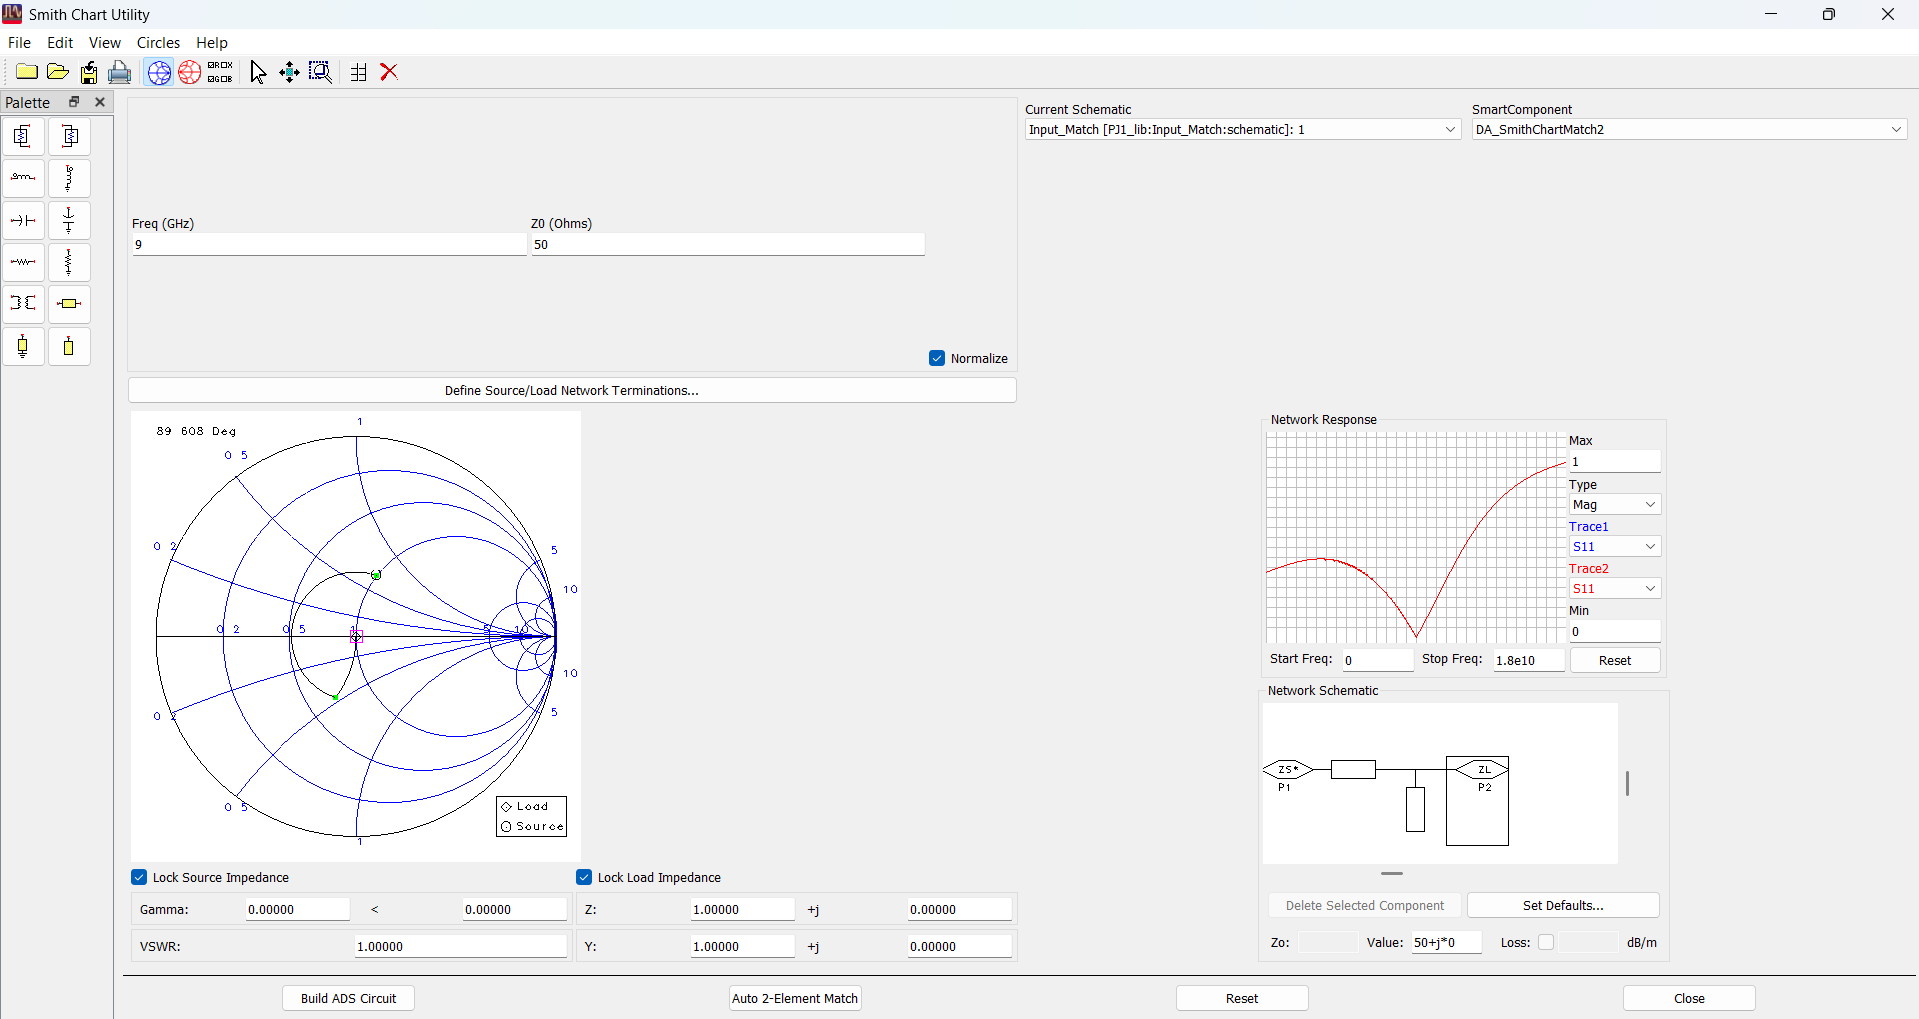
\includegraphics[width=0.8\textwidth]{./img/smith_chart_output.png}
		\caption{محیط طراحی شبکه تطبیق خروجی در ابزار \lr{Smith Chart} نرم‌افزار \lr{ADS}؛ توپولوژی شامل یک خط انتقال سری و یک استاب موازی مدار باز است}
		\label{fig:smith_output}
	\end{figure}
	
	بعد از تکمیل موفق هر دو مسیر طراحی و اطمینان از تطبیق، با استفاده از گزینه \lr{Build ADS Circuit}، نرم‌افزار این طراحی‌ها را به‌صورت بلوک‌های آماده اسمیت چارت (\lr{SmartComponent}) تولید کرد و به محیط شماتیک اصلی منتقل کرد. نمای کلی شماتیک نهایی که شامل هر دو شبکه (ورودی و خروجی) و اتصالاتشان است، در شکل \ref{fig:schematic_smith} قابل مشاهده است.
	
	\begin{figure}[htbp]
		\centering
		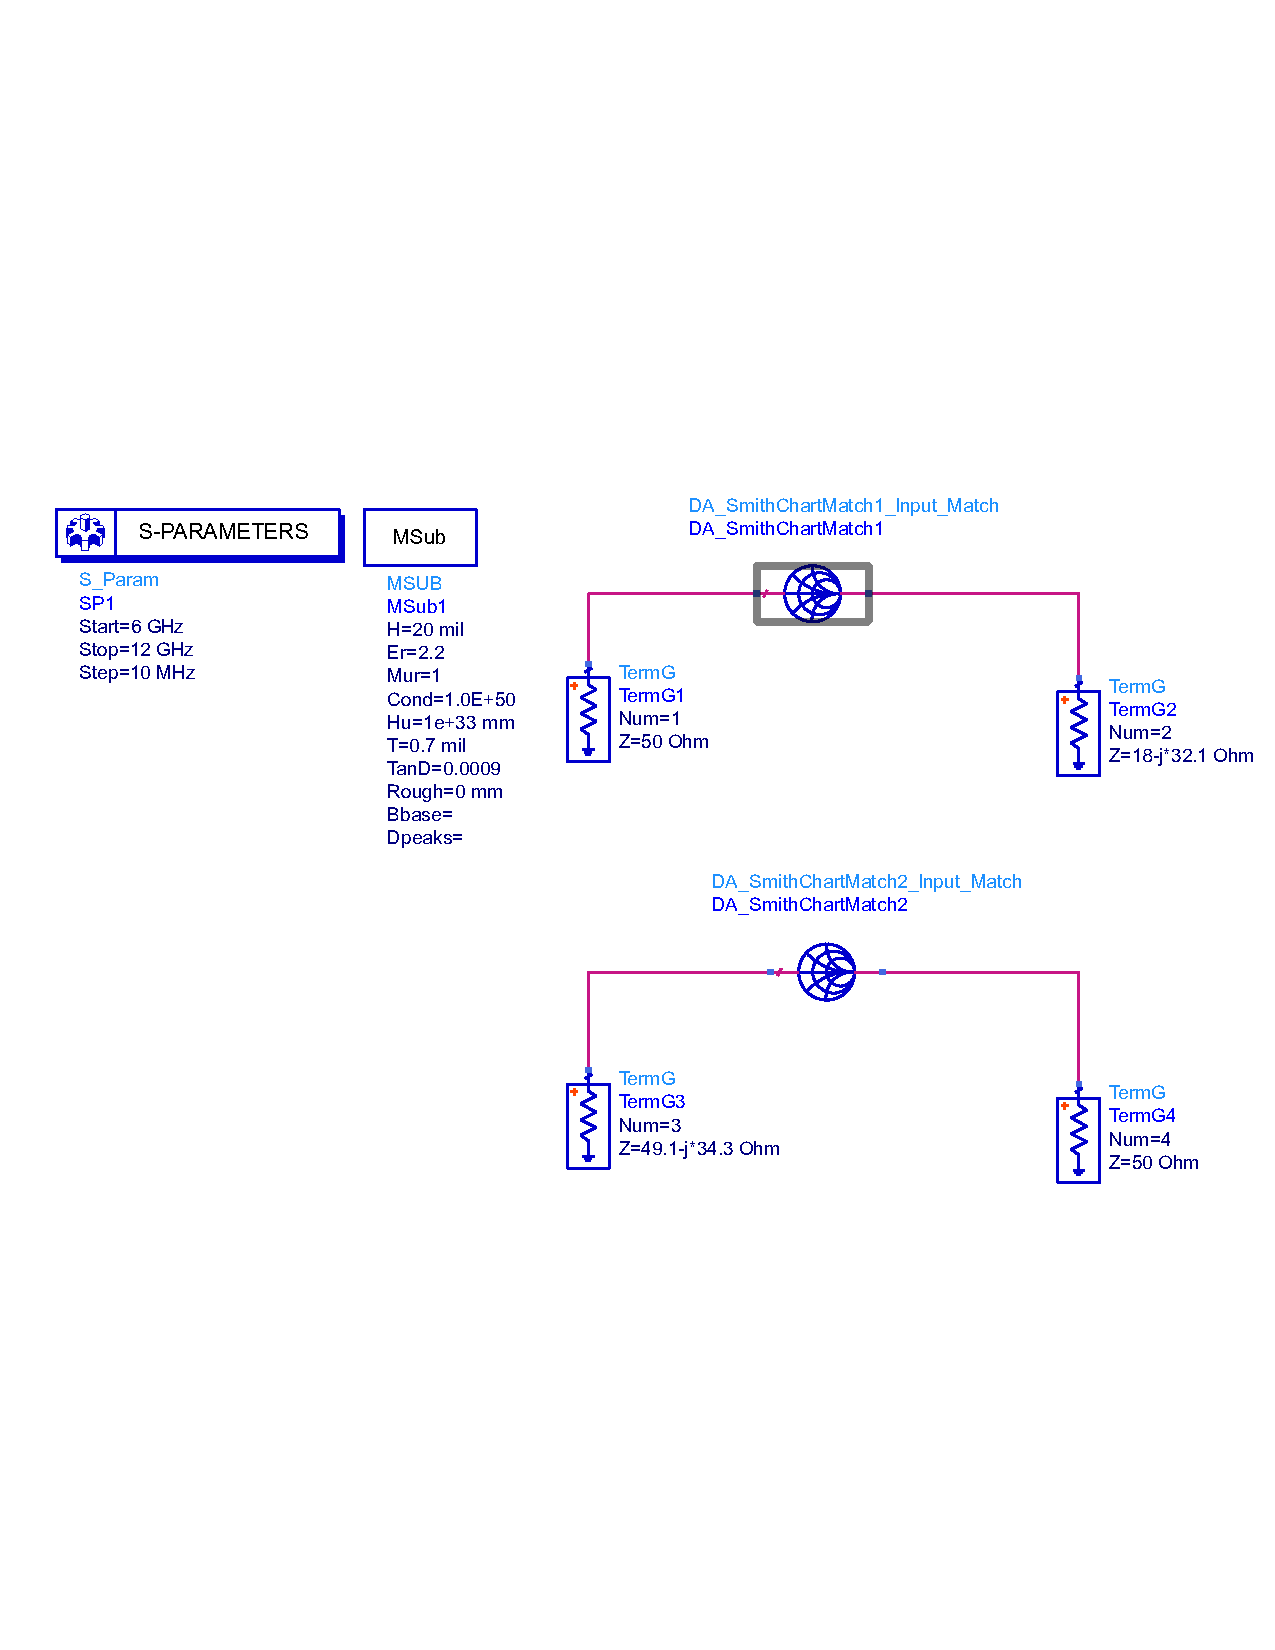
\includegraphics[trim=0 7.5cm 0 8.4cm, clip,width=0.8\textwidth]{./img/test.pdf}
		\caption{شماتیک مدار شبکه‌های تطبیق ورودی و خروجی با استفاده از بلوک‌های اسمیت چارت و خطوط انتقال}
		\label{fig:schematic_smith}
	\end{figure}
	
	\subsection{نتایج شبیه‌سازی و اعتبارسنجی نهایی مدل ایده‌آل}
	
	بعد از اجرای شبیه‌سازی در بازه فرکانسی ۶ تا ۱۲ گیگاهرتز، نتایج پارامترهای پراکندگی مدار کامل را استخراج کردم. نتایج نشان می‌دهند که شبکه تطبیق ورودی عملکرد خیلی خوبی داشته و در فرکانس مرکزی ۹ گیگاهرتز، پارامتر $S_{11}$ به مقدار $-48.213\ \text{dB}$ رسیده است. شبکه تطبیق خروجی هم رزونانس مناسبی را در فرکانس کاری تجربه کرده؛ به‌طوری‌که پارامتر $S_{33}$ در فرکانس ۹ گیگاهرتز مقدار $-42.618\ \text{dB}$ را نشان می‌دهد.
	
	نمودار اسمیت هم این تطبیق دقیق را تأیید می‌کند؛
	
	\begin{figure}[htbp]
		\centering
		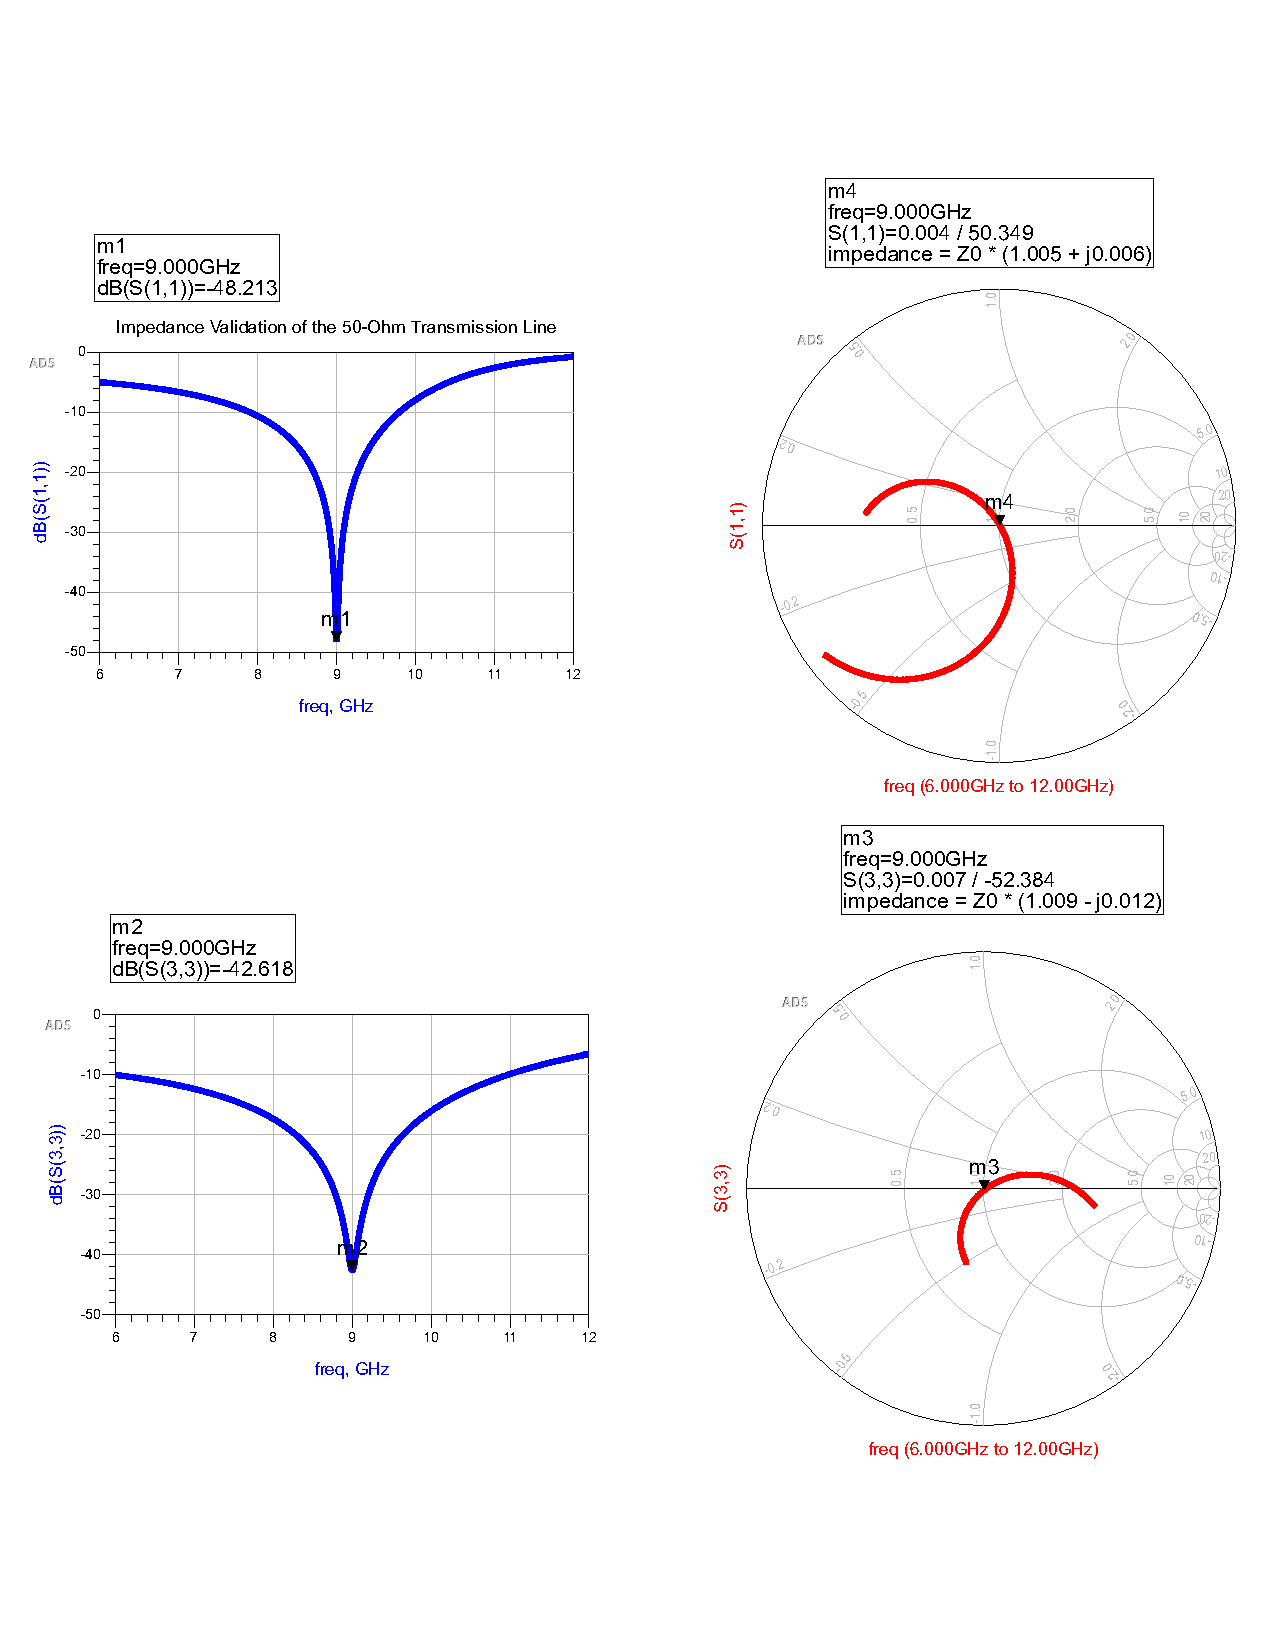
\includegraphics[trim=0 3.8cm 0 3cm, clip,width=0.8\textwidth]{./img/test_chematic.pdf}
		\caption{نتایج شبیه‌سازی شبکه‌های تطبیق: نمودار اندازه پارامترهای پراکندگی و نمودار اسمیت}
		\label{fig:results_smith}
	\end{figure}
	
	\subsection{از بلوک آرمانی اسمیت چارت به خط واقعی مایکرواستریپ}
	
	بعد از سنتز شبکه‌های تطبیق ورودی و خروجی در محیط ایده‌آل ابزار \lr{Smith Chart} و به‌دست آوردن امپدانس مشخصه و طول الکتریکی لازم برای هر یک از عناصر (خط انتقال سری و استاب موازی مدار باز)، نوبت به پیاده‌سازی فیزیکی این عناصر با خطوط مایکرواستریپ رسید. برای این کار، از همان زیرلایه \lr{RT5880} با مشخصات معرفی‌شده در بخش قبل ($\varepsilon_r=2.2$، $H=20\ \text{mil}$، $T=0.7\ \text{mil}$، $\tan\delta=0.0009$) استفاده کردم و با کمک ابزار \lr{LineCalc} نرم‌افزار \lr{ADS}، امپدانس مشخصه و طول الکتریکی هر قطعه را در فرکانس کاری ۹ گیگاهرتز به عرض ($W$) و طول فیزیکی ($L$) متناظر نوار مایکرواستریپ تبدیل کردم.
	
	\subsubsection{دوباره \lr{LineCalc}، این‌بار با احتیاط بیشتر}
	
	این‌بار با درسی که از خطای واحد بخش قبل گرفته بودم، هر مقدار خروجی \lr{LineCalc} را قبل از وارد کردن در فیلد \lr{L} یا \lr{W} یک‌بار دیگر با واحدش چک کردم. عرض محاسبه‌شده برای تمام قطعات (خطوط سری و استاب‌ها)، با توجه به امپدانس مشخصه مرجع ۵۰ اهمی، برابر با $W = 60.770079\ \text{mil}$ به دست آمد که با عرض محاسبه‌شده در بخش اعتبارسنجی خط انتقال ۵۰ اهمی (ابتدای گزارش) کاملاً مطابقت دارد که خودش یک تأیید غیرمستقیم خوب بود. طول فیزیکی هر یک از چهار قطعه سنتزشده در جدول \ref{tab:linecalc_dims} آمده است.
	
	\begin{table}[H]
		\centering
		\caption{ابعاد فیزیکی عناصر مایکرواستریپ شبکه‌های تطبیق، محاسبه‌شده با \lr{LineCalc}}
		\label{tab:linecalc_dims}
		\begin{tabular}{|c|c|c|c|c|}
			\hline
			\textbf{شبکه} & \textbf{نقش قطعه} & \textbf{نام قطعه} & \textbf{عرض $W$ (mil)} & \textbf{طول $L$ (mil)} \\
			\hline
			ورودی & استاب موازی مدار باز (\lr{MLOC}) & \lr{TL3} & $60.770079$ & $149.920079$ \\
			\hline
			ورودی & خط انتقال سری (\lr{MLIN}) & \lr{TL4} & $60.770079$ & $163.558661$ \\
			\hline
			خروجی & خط انتقال سری (\lr{MLIN}) & \lr{TL5} & $60.770079$ & $237.770472$ \\
			\hline
			خروجی & استاب موازی مدار باز (\lr{MLOC}) & \lr{TL6} & $60.770079$ & $90.538583$ \\
			\hline
		\end{tabular}
	\end{table}
	
	\subsubsection{شماتیک نهایی و اولین نتایج امیدوارکننده}
	
	چیدمان نهایی این عناصر به همراه ترمینال‌های مرجع (\lr{TermG}) در شکل \ref{fig:real_schematic} دیده می‌شود. در این شماتیک، برای این‌که بتوانم هر شبکه را به‌طور مستقل و دقیق اعتبارسنجی کنم (بدون نیاز به مدل کامل ترانزیستور)، پورت‌های \lr{Num=1} و \lr{Num=4} را با امپدانس مرجع $50\ \Omega$ گذاشتم و پورت‌های \lr{Num=2} و \lr{Num=3} را مستقیماً با مقدار دقیق امپدانس ورودی ($18-j32.1\ \Omega$) و خروجی ($49.1-j34.3\ \Omega$) ترانزیستور ختم کردم.
	
	\begin{figure}[H]
		\centering
		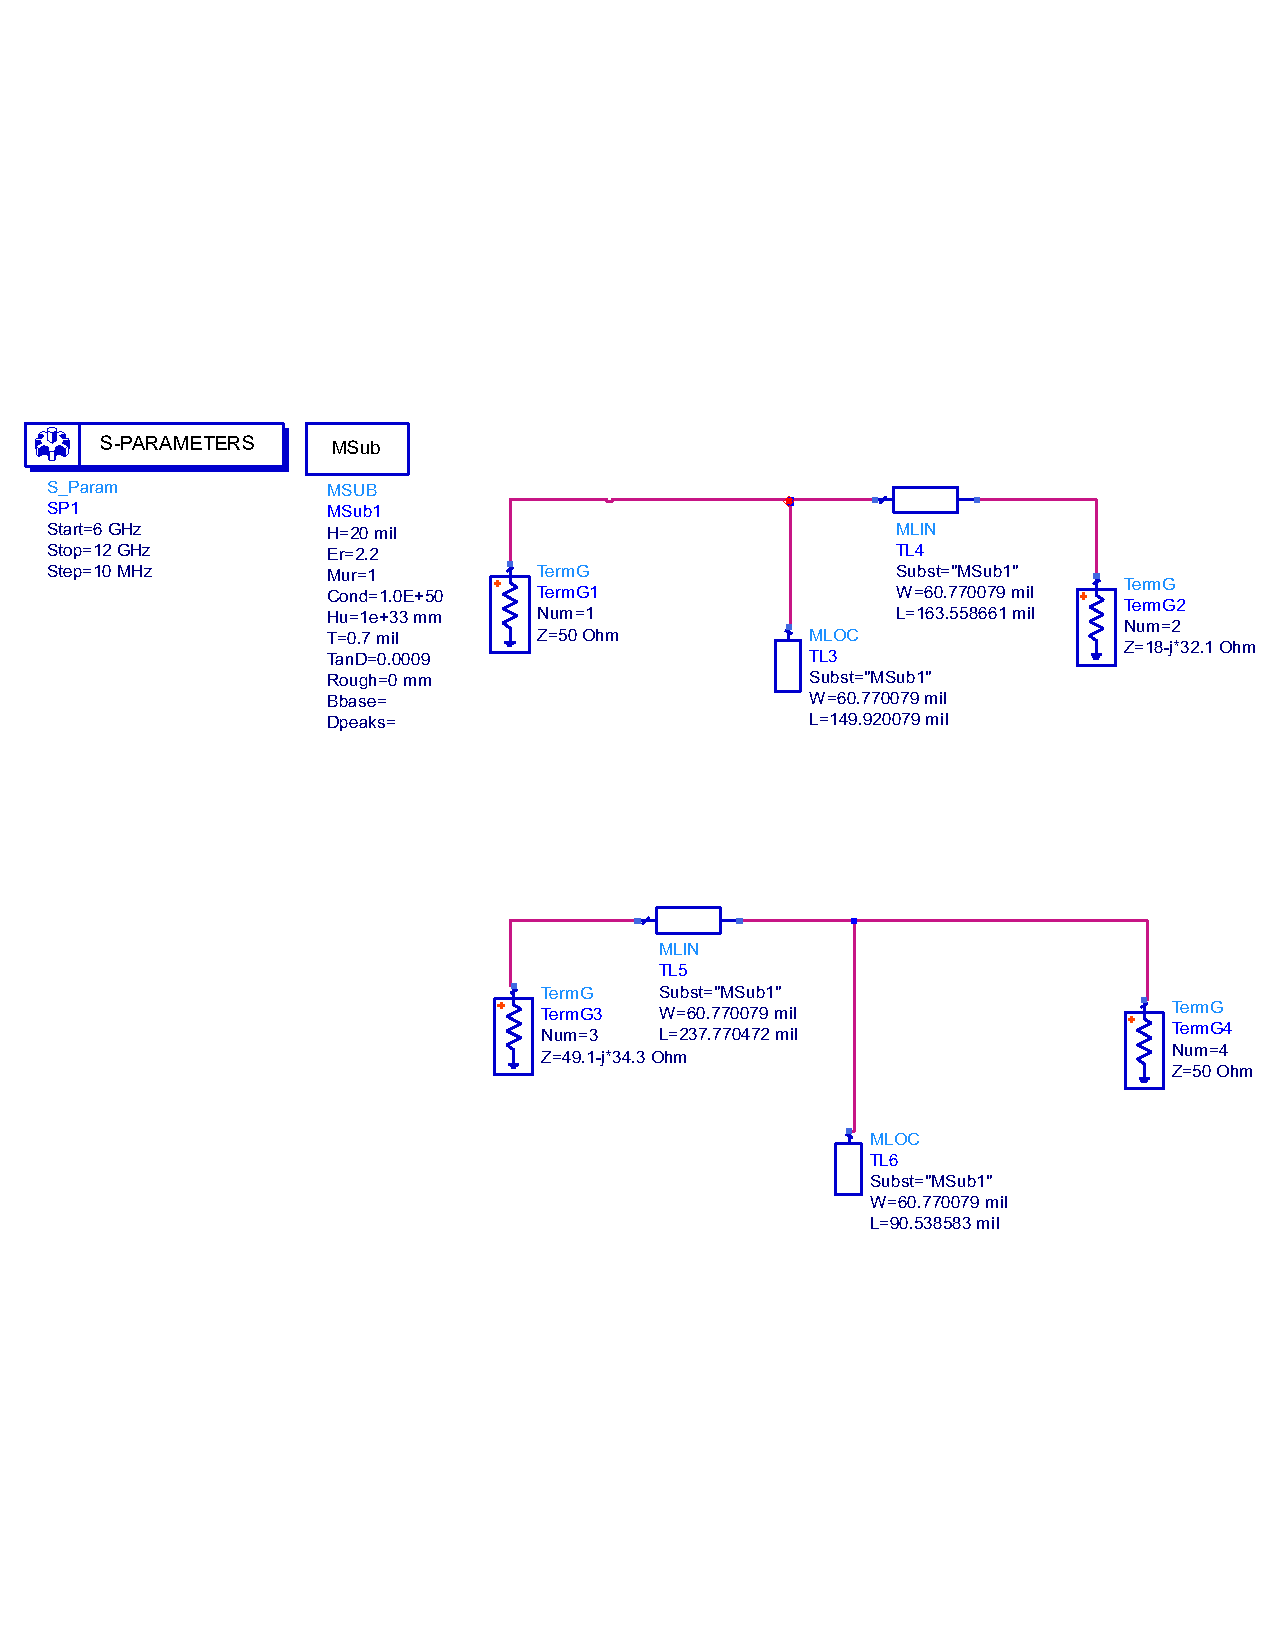
\includegraphics[trim = 0cm 7cm 0cm 7cm, clip,width=0.8\textwidth]{./img/real_shematic.pdf}
		\caption{شماتیک نهایی پیاده‌سازی فیزیکی شبکه‌های تطبیق ورودی و خروجی با عناصر مایکرواستریپ \lr{MLIN}/\lr{MLOC}}
		\label{fig:real_schematic}
	\end{figure}
	
	شبیه‌سازی پارامترهای پراکندگی این مدار را در بازه فرکانسی ۶ تا ۱۲ گیگاهرتز و با گام فرکانسی $\text{Step}=10\ \text{MHz}$ دوباره اجرا کردم. نتایج نشان می‌دهند که در فرکانس مرکزی ۹ گیگاهرتز، شبکه تطبیق ورودی به مقدار $S_{11} = -59.463\ \text{dB}$ رسیده و امپدانس نرمالیزه دیده‌شده از پورت ۱ برابر با $0.998 + j6.856\times10^{-5}$ است؛ این مقدار عملاً برابر با $1$ است و یعنی تطبیق تقریباً کامل با مرجع $50\ \Omega$ اتفاق افتاده. شبکه تطبیق خروجی هم عملکرد خیلی خوبی داشته و در همین فرکانس، $S_{33} = -42.497\ \text{dB}$ به دست آمده.
	
	جالب این‌جاست که این مقادیر، در مقایسه با نتایج مدل ایده‌آل ابزار \lr{Smith Chart} (بخش قبل)، یک تفاوت جزئی دارند که کاملاً منطقی است: این تفاوت از گرد کردن ابعاد فیزیکی به مقادیر استاندارد قابل‌ساخت و اثرات واقعی خط مایکرواستریپ (از جمله پاشندگی و تلفات دی‌الکتریک زیرلایه) نسبت به مدل آرمانی خط انتقال ایده‌آل می‌آید. با این حال، هر دو مقدار به‌طور قابل‌توجهی کمتر از آستانه معمول $-20\ \text{dB}$ برای تطبیق قابل‌قبول هستند و صحت طراحی فیزیکی شبکه‌های تطبیق را تأیید می‌کنند. نمودارهای مربوط به این نتایج در شکل \ref{fig:real_results} آورده شده‌اند.
	
	\begin{figure}[H]
		\centering
		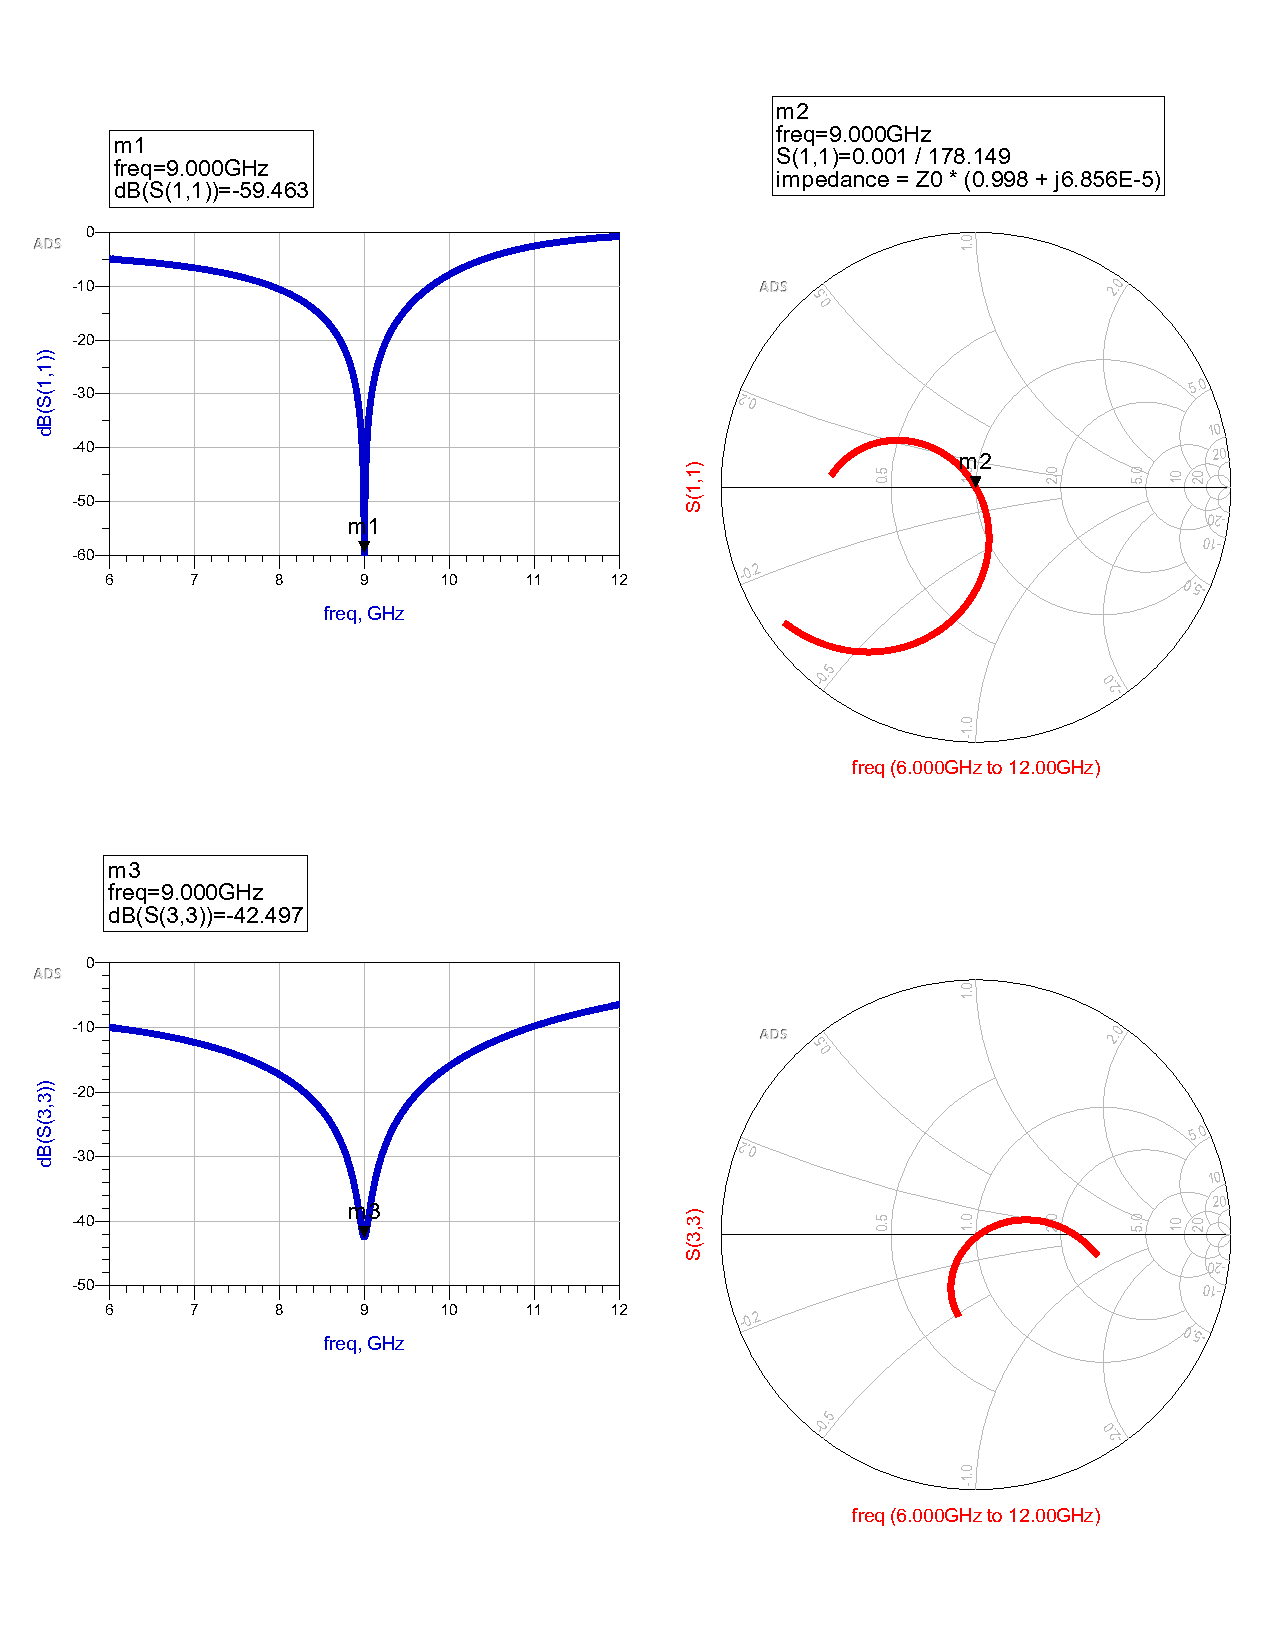
\includegraphics[trim = 0cm 2cm 0cm 1.5cm, clip, width=0.8\textwidth]{./img/real_output.pdf}
		\caption{نتایج شبیه‌سازی پیاده‌سازی فیزیکی شبکه‌های تطبیق: نمودار اندازه $S_{11}$ و $S_{33}$ و نمودار اسمیت متناظر}
		\label{fig:real_results}
	\end{figure}
	
	\subsection{یک نکته دقیق‌تر: اتصال \texorpdfstring{\lr{T}}{T} در محل پیوستن استاب کجاست؟}
	
	با این‌که نتایج بخش قبل خودشان کاملاً قابل قبول بودند، یک نکته فیزیکی وجود داشت که در شماتیک قبلی نادیده گرفته شده بود: در آن شماتیک، خط انتقال سری و استاب موازی مدار باز، دقیقاً روی هم و در یک نقطه به هم وصل شده بودند، طوری که \lr{ADS} این پیوستگی را به‌صورت یک اتصال ایده‌آل و بدون هیچ اثر پارازیتی در نظر می‌گرفت. اما در واقعیت، هر جا که سه خط مایکرواستریپ (خط ورودی، خط خروجی و استاب) به هم می‌رسند، یک \textbf{ناپیوستگی سه‌راهی} (\lr{T-Junction}) شکل می‌گیرد که خودش یک اثر رآکتیو اضافه با خودش می‌آورد؛ همان چیزی که در بخش تلفات و ناپیوستگی‌ها هم به آن اشاره شد.
	
	برای این‌که این اثر را هم در شبیه‌سازی لحاظ کنم، به سراغ کتابخانه قطعات \lr{ADS} رفتم و به‌جای اتصال مستقیم سه خط به هم، از قطعه آماده \lr{MTEE\_ADS} استفاده کردم که دقیقاً مدل سه‌راهی مایکرواستریپ را با در نظر گرفتن عرض هر سه بازو پیاده می‌کند. در شماتیک نهایی، دو بلوک \lr{MTEE\_ADS} با نام‌های \lr{Tee1} (برای شبکه ورودی) و \lr{Tee2} (برای شبکه خروجی) جایگزین محل تلاقی خط سری و استاب شدند؛ شکل \ref{fig:final_schematic} این چیدمان نهایی را نشان می‌دهد.
	
	طبیعتاً همین‌که مدل دقیق‌تر \lr{T-Junction} وارد مدار شد، طول‌های قبلی که از \lr{LineCalc} به دست آمده بودند دیگر دقیقاً نقطه بهینه نبودند چون آن طول‌ها برای یک اتصال ایده‌آل محاسبه شده بودند، نه برای یک ناپیوستگی واقعی با سوسپتانس اضافه. برای همین یک دور دیگر \lr{Optimization} روی طول چهار قطعه \lr{TL3} تا \lr{TL6} اجرا کردم تا مدار با حضور بلوک‌های \lr{MTEE} دوباره درست تنظیم شود. طول‌های نهایی بعد از این دور بهینه‌سازی در جدول \ref{tab:final_dims} آمده‌اند؛ همان‌طور که دیده می‌شود، تفاوتشان با طول‌های اولیه \lr{LineCalc} (جدول \ref{tab:linecalc_dims}) چندان زیاد نیست، اما همین اصلاح کوچک برای جبران اثر واقعی \lr{T-Junction} لازم بود.
	
	\begin{figure}[H]
		\centering
		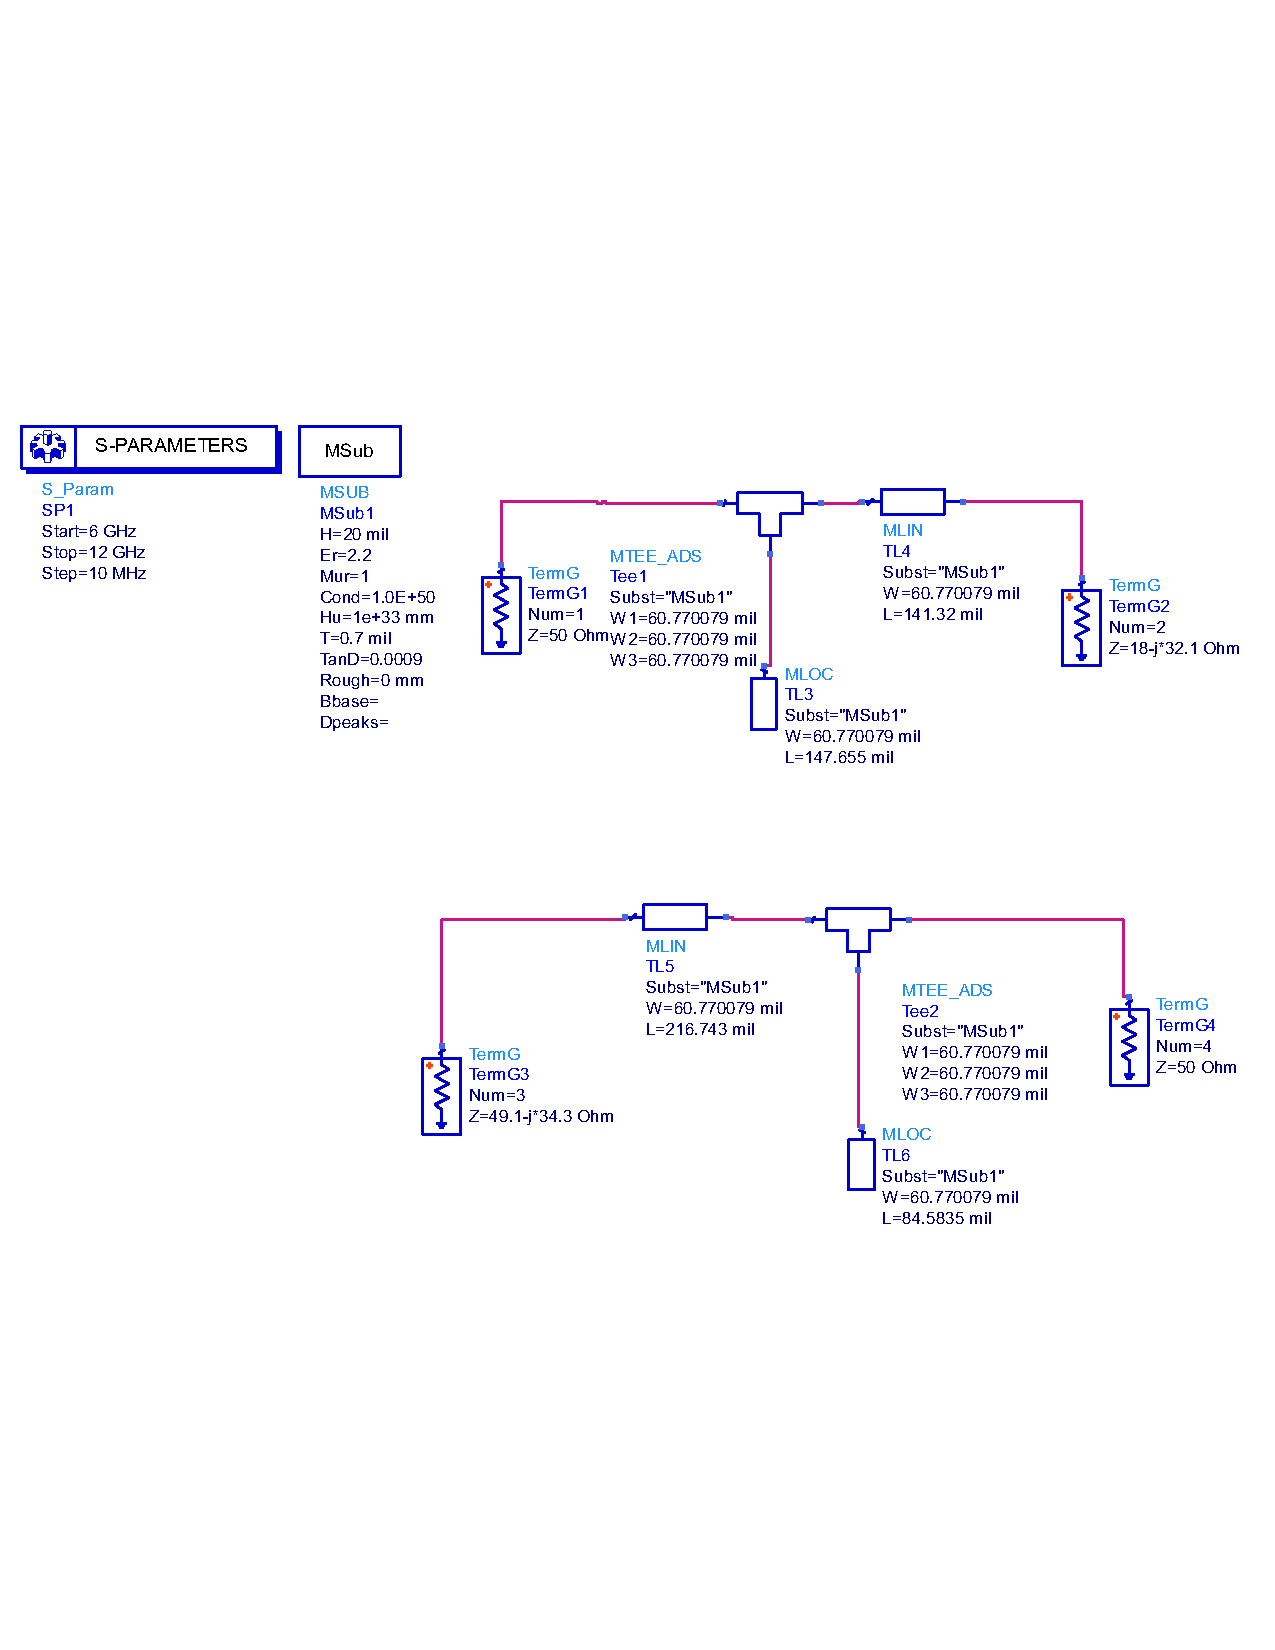
\includegraphics[trim = 0cm 7cm 0cm 7cm, clip,width=0.9\textwidth]{./img/final_shematic.pdf}
		\caption{شماتیک نهایی شبکه‌های تطبیق با بلوک‌های \lr{MTEE\_ADS} در محل اتصال سه‌راهی، بعد از دور دوم بهینه‌سازی}
		\label{fig:final_schematic}
	\end{figure}
	
	\begin{table}[H]
		\centering
		\caption{طول‌های نهایی قطعات مایکرواستریپ بعد از اضافه‌شدن \lr{MTEE} و بهینه‌سازی دوباره}
		\label{tab:final_dims}
		\begin{tabular}{|c|c|c|c|}
			\hline
			\textbf{نقش قطعه} & \textbf{نام قطعه} & \textbf{عرض $W$ (mil)} & \textbf{طول $L$ (mil)} \\
			\hline
			استاب موازی مدار باز (ورودی) & \lr{TL3} & $60.770079$ & $147.655$ \\
			\hline
			خط انتقال سری (ورودی) & \lr{TL4} & $60.770079$ & $141.32$ \\
			\hline
			خط انتقال سری (خروجی) & \lr{TL5} & $60.770079$ & $216.743$ \\
			\hline
			استاب موازی مدار باز (خروجی) & \lr{TL6} & $60.770079$ & $84.5835$ \\
			\hline
		\end{tabular}
	\end{table}
	
	\subsection{از شماتیک تا \lr{Layout}: دردسر لایه‌ها و شبیه‌سازی \lr{Momentum}}
	
	با طول‌های اصلاح‌شده و بلوک‌های \lr{MTEE} در محل خودشان، مدار از حالت تئوری کاملاً خارج شد و به فرم فیزیکی مایکرواستریپ کامل تبدیل شد. در این مرحله، شبکه‌های تطبیق با استفاده از خطوط سری (\lr{MLIN})، استاب‌های موازی (\lr{MLOC}) و همان سه‌راهی‌های \lr{MTEE} که در بخش قبل توضیح دادم، روی زیرلایه با ثابت دی‌الکتریک $2.2$ و ضخامت $20\text{ mil}$ پیاده‌سازی شدند.
	
	برای بررسی ساختار فیزیکی پیش از ساخت واقعی، مدار را به محیط \lr{Layout} منتقل کردم
	
	شکل‌های \ref{fig:layout_2d} و \ref{fig:layout_3d} به ترتیب نمای دوبعدی شبکه‌های تطبیق ورودی و خروجی (که حالا شامل بلوک‌های \lr{MTEE} هم می‌شوند) و نمای سه‌بعدی نهایی برد چاپ‌شده (\lr{PCB}) را نشان می‌دهند. همان‌طور که دیده می‌شود، مسیرهای مسی کاملاً یکپارچه‌اند و پورت‌های ورودی و خروجی به‌درستی روی لبه‌های مدار جای گرفته‌اند.
	
	\begin{figure}[H]
		\centering
		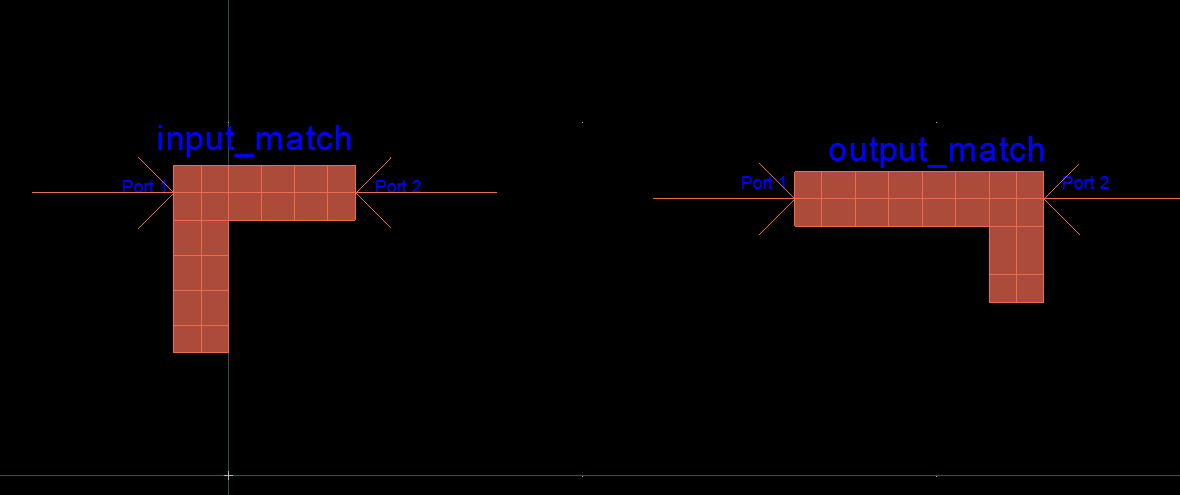
\includegraphics[width=1\textwidth]{./img/momentom_chematic.png}
		\caption{نمای دوبعدی شبکه‌های تطبیق در محیط \lr{Layout} نرم‌افزار \lr{ADS}، بعد از اصلاح نگاشت لایه‌ها}
		\label{fig:layout_2d}
	\end{figure}
	
	\begin{figure}[H]
		\centering
		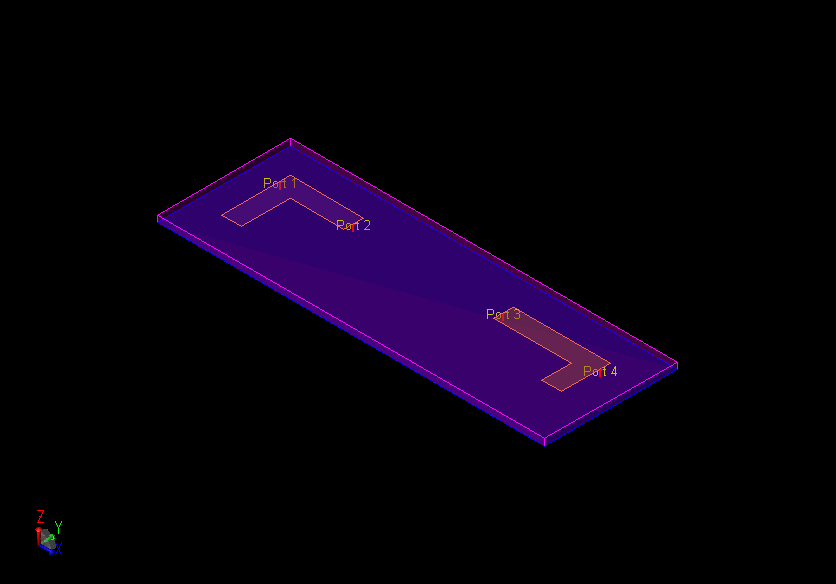
\includegraphics[width=1\textwidth]{./img/pcb.png}
		\caption{نمای سه‌بعدی برد فیزیکی (\lr{PCB}) نهایی در محیط \lr{Momentum}}
		\label{fig:layout_3d}
	\end{figure}
	
	بعد از رفع این مشکل، برای اعتبارسنجی دقیق عملکرد مدار فیزیکی و در نظر گرفتن تمام اثرات پارازیتی، تزویج متقابل بین خطوط، اثر واقعی سه‌راهی‌های \lr{MTEE}، و تلفات هادی و دی‌الکتریک، شبیه‌سازی تمام‌موج الکترومغناطیسی (\lr{Momentum}) را روی این ساختار اجرا کردم. نتایج این شبیه‌سازی شامل اندازه پارامترهای پراکندگی، فاز و نمودار اسمیت در شکل‌های \ref{fig:momentum_mag} و \ref{fig:momentum_smith} آورده شده است.
	
	بر اساس نمودارهای استخراج‌شده، مدار طراحی‌شده در فرکانس مرکزی $9\text{ GHz}$ عملکرد خیلی خوبی از خودش نشان می‌دهد؛ پارامترهای انعکاس شبکه (یعنی $S_{11}$، $S_{22}$، $S_{33}$ و $S_{44}$) دقیقاً در همین فرکانس افت شدیدی دارند و کاملاً تشدید شده‌اند. این نتیجه تأیید می‌کند که هم مدل کردن دقیق سه‌راهی‌ها با \lr{MTEE}، هم بهینه‌سازی دوباره طول خطوط، و هم رفع مشکل نگاشت لایه‌ها همگی موفقیت‌آمیز بوده‌اند و تطبیق امپدانس عالی حتی در حضور فیزیک واقعی مدار هم محقق شده است.
	
	\begin{figure}[htbp]
		\centering
		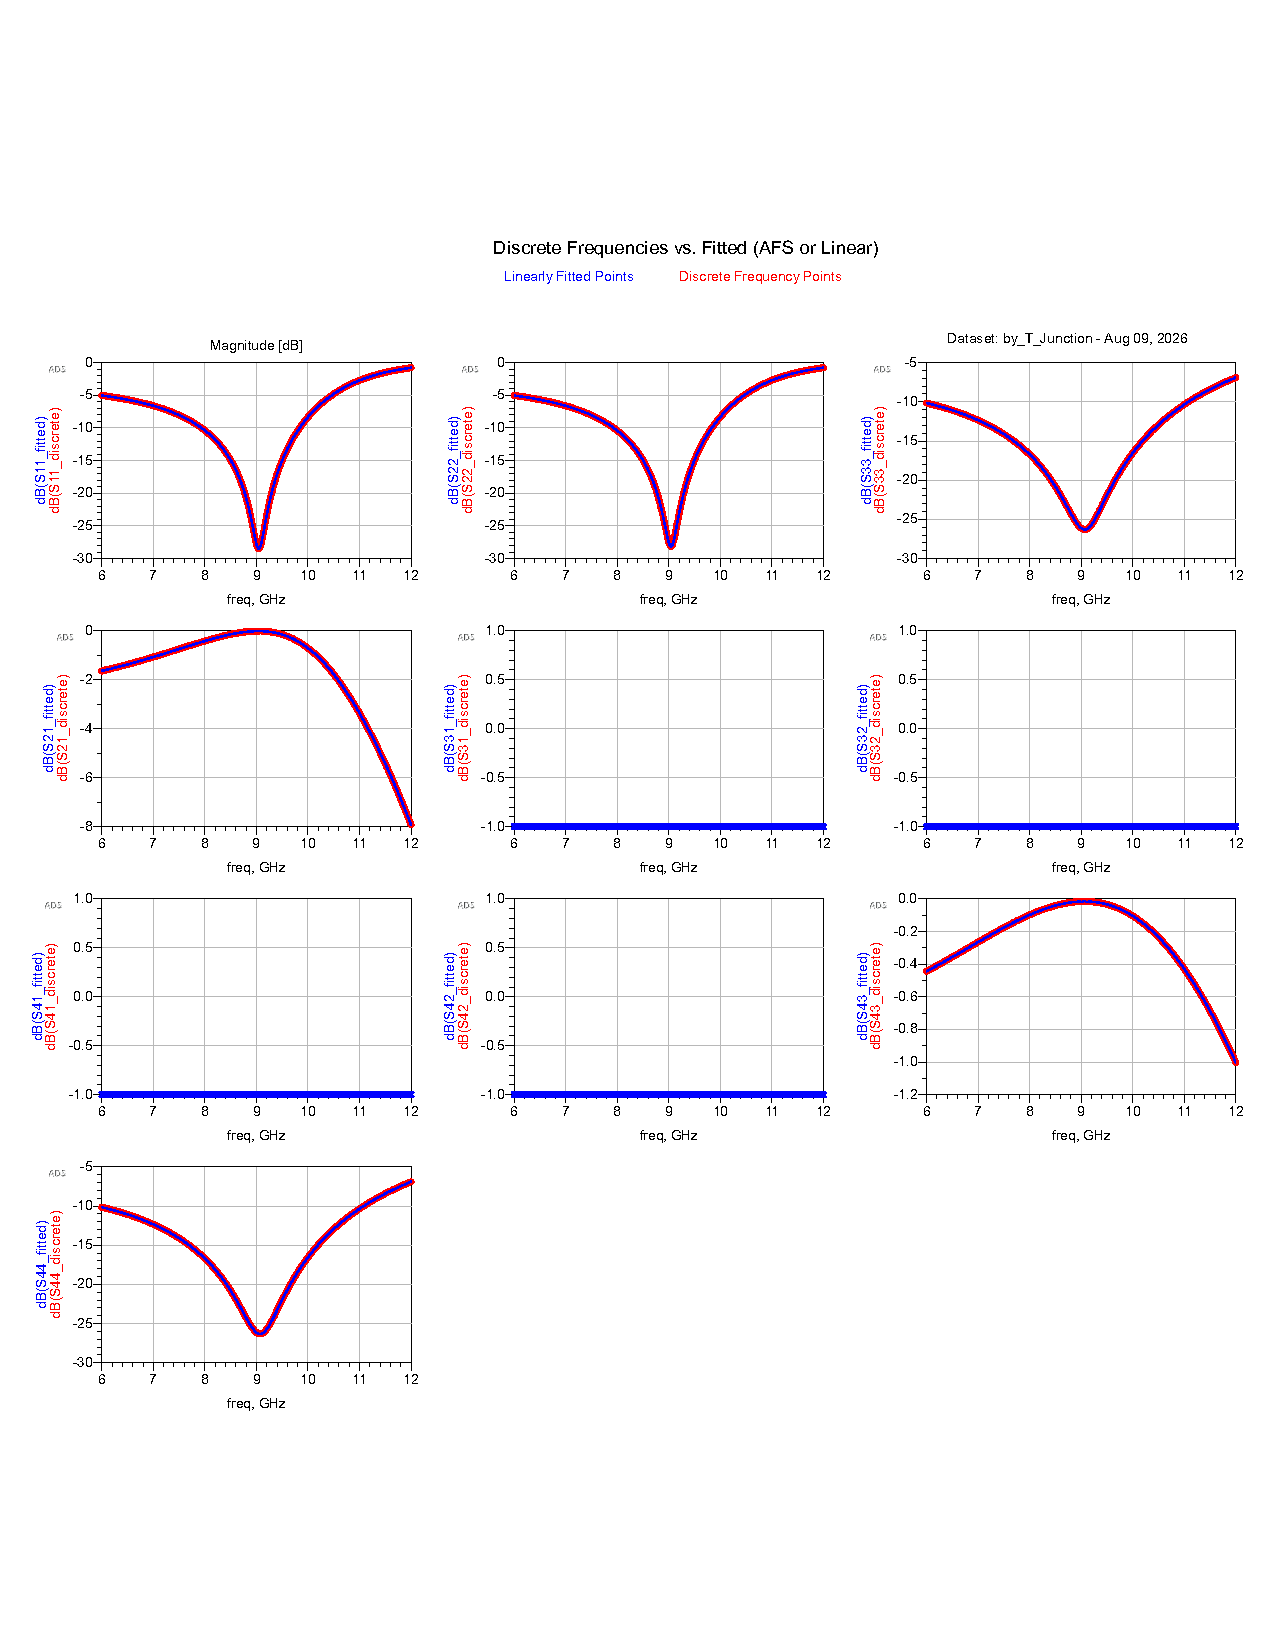
\includegraphics[trim = 0cm 2cm 0cm 2cm, clip, width=1.05\textwidth]{./img/momentom_s.pdf}
		\caption{اندازه پارامتر های پراکندگی در شبیه سازی ممنتوم}
		\label{fig:momentum_mag}
	\end{figure}
	
	
	\begin{figure}[htbp]
		\centering
		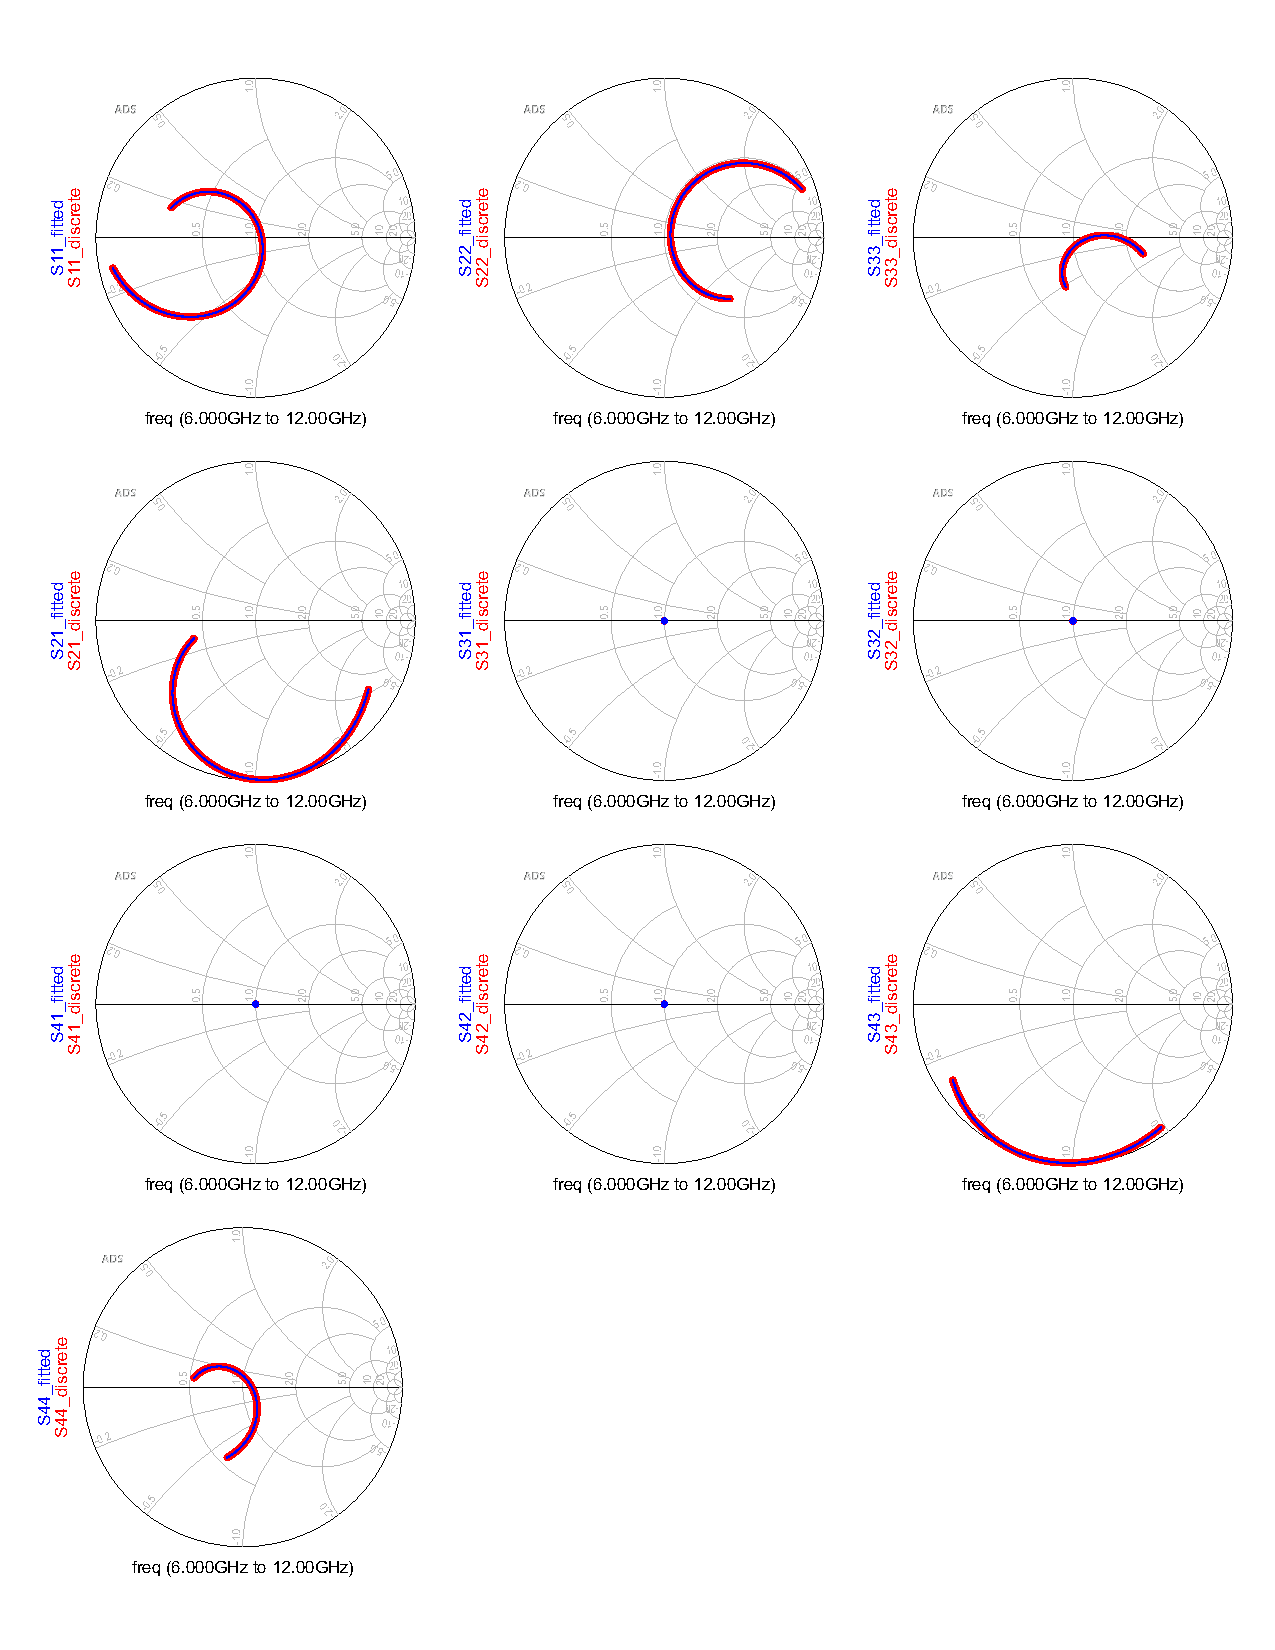
\includegraphics[trim = 0cm 1.2cm 0cm 1.cm, clip, width=1.05\textwidth]{./img/momentom_smith_chart.pdf}
		\caption{نمودار اسمیت پارامتر های پراکندگی در شبیه سازی ممنتوم}
		\label{fig:momentum_smith}
	\end{figure}
	

\end{document}